\documentclass[a4paper]{article}

%% Language and font encodings
\usepackage[english]{babel}
\usepackage[utf8x]{inputenc}
\usepackage[T1]{fontenc}
\usepackage{booktabs}
\usepackage{multirow}

%% Sets page size and margins
\usepackage[a4paper,top=3cm,bottom=2cm,left=3cm,right=3cm,marginparwidth=1.75cm]{geometry}

%% Useful packages
\usepackage{amsmath}
\usepackage{graphicx}
\usepackage[colorinlistoftodos]{todonotes}
\usepackage[colorlinks=true, allcolors=blue]{hyperref}
\usepackage{siunitx}
% \usepackage{subfigure}
\usepackage{subcaption}


\graphicspath{{_fig_optical/}}

\title{Electron-neutrino reconstruction in MicroBooNE using the Pandora reconstruction framework}
\author{The MicroBooNE collaboration}

\begin{document}
\maketitle
\tableofcontents

\begin{abstract}
MicroBooNE (the Micro Booster Neutrino Experiment) is a liquid argon
time-projection chamber experiment designed for short-baseline neutrino physics, currently running at Fermilab. It aims to address the anomalous excess of low-energy events observed by the previous MiniBooNE experiment. In this note we demonstrate the ability of the experiment to reconstruct electron neutrino-like events in the detector, using the Pandora reconstruction framework. In particular, we present a fully automated event selection algorithm that can identify charged-current electron neutrino event candidates with no pions and at least one proton in the final state.
\end{abstract}


\section{Introduction}
One of the main physics goals of the MicroBooNE experiment is to clarify the nature of the low-energy excess of $\nu_{e}$-like events observed by the MiniBooNE experiment in 2009. The excess was found in the neutrino energy region between 200 to 475 MeV in 2009.

However, the MiniBooNE detector was a \v{C}erenkov detector, which is not able to distinguish between single electrons and single photons in the final state, making it impossible to pick a physics model among those which could explain the excess.

The MicroBooNE detector, instead, is a liquid argon time projection chamber. This technology provides detailed tracking and allows to measure the rate of energy loss per track length of each particle ($dE/dx$), which is essential for electron/photon identification.

In this note we will describe an algorithm which aims to select $\nu_{e}$ interactions in the MicroBooNE detector in a $\nu_{\mu}$ beam, such as the Booster Neutrino Beam (BNB) at the Fermi National Accelerator Laboratory.

\section{Signal definition}
The Standard Model, at tree level, allows only weak interaction for neutrinos. As such, neutrinos exchange a $W^{\pm}$ vector boson in charged-current (CC) interactions and a $Z$ vector boson in neutral-current (NC) interactions. 
However, the energy of a neutrino can range from few keV to several PeV, as recently measured by the IceCube experiment \cite{icecube}, producing wildly different topologies in the final state. 
In our case, we are interested in $\nu_{e}$ CC interactions in the sub-GeV region (0.1 - 1~GeV). In a naive scenario, where we ignore nuclear and final-state interactions, we can have three dominant outcomes:
\begin{itemize}
\item Charged Current Quasi Elastic (CCQE): it is the principal signature for most neutrino experiments. The neutrino exchanges a $W^{\pm}$ with a neutron, producing a proton and a charged lepton in the final state.
\item Charged Current Resonant production (CCRES): the neutrino excites a nucleon, which emits a pion.
\item Charged Current Deep Inelastic Scattering (CCDIS): the neutrino interacts with a quark, producing a shower of particles as the nucleus breaks apart.
\end{itemize}

However, hadrons exiting the nucleus after the neutrino interaction can re-interact and change identity or eject other hadrons (Final State Interactions, FSI) \cite{ccqe2}. It is then necessary to define the signal by the particles in its final state. Our selection aims to have a sample with one electron, no other leptons or photons, at least one proton, and no other hadrons or mesons. This kind of event is called CC0$\pi$-Np (where N > 0) \cite{teppei}.

In a LArTPC, the final state of a contained $\nu_{e}$ CC0$\pi$-Np interaction will correspond in general to one or more ionisation tracks, produced by the protons, and an electromagnetic shower, produced by the electron. A charged pion in the final state, instead, will decay mainly into a muon, producing a second ionisation track, while a neutral pion will decay into two photons, producing two electromagnetic showers. 
CCDIS interactions, whose branching ratio is relatively small in the sub-Gev region, usually produce large hadronic jets, which are reconstructed as a combination of tracks and showers. 

%As such, a perfect reconstruction of a $\nu_{e}$ CCQE-like event in a LArTPC will produce as many ionisation tracks as the number of protons in the final state and a single electromagnetic shower (the electron), sharing a common vertex.

The MiniBooNE experiment showed an excess of CCQE-like events (one proton and one electron in the final state) in the 200-475~MeV neutrino energy range \cite{miniboone}, so our analysis will focus on a similar topology in an analogous energy range.

\section{The selection algorithm}
In the TPC, ionisation electrons passing through the MicroBooNE cryostat are drifted to the anode, inducing electric signals on the wires of the three TPC planes. The waveforms observed for each wire are examined and a hit-finding algorithm searches for local maxima and minima. A Gaussian distribution is fitted to each peak and hit objects are created. The hits are used by the reconstruction algorithms provided by the Pandora framework \cite{pandora} to form TPC reconstructed objects. 

The Pandora reconstruction produces as a first stage a list of two-dimensional clusters, which represent continuous, unambiguous lines of hits. Thus, cluster-merging algorithms identify associations between multiple clusters. The three-dimensional track and shower reconstruction then collects the two-dimensional clusters from the three readout planes that represent individual, track-like or shower-like objects \cite{pandora2}. Our analysis relies on these high-level reconstructed objects to select our CC0$\pi$-Np candidates.

MicroBooNE is also equipped with an optical system made of 32 photomultipliers tubes placed behind the anode plane, with few-ns timing resolution. The optical system detects the argon scintillation light produced by the neutrino interaction and it provides the TPC start time of the event.
Figure \ref{fig:evd} shows a simulated event display of one wire plane with an electron and two protons in the final state, with the corresponding reconstructed shower and reconstructed tracks. In this case, the algorithm was able to correctly reconstruct the electromagnetic shower and both proton tracks.

\begin{figure}[htbp]
	\begin{center}
    	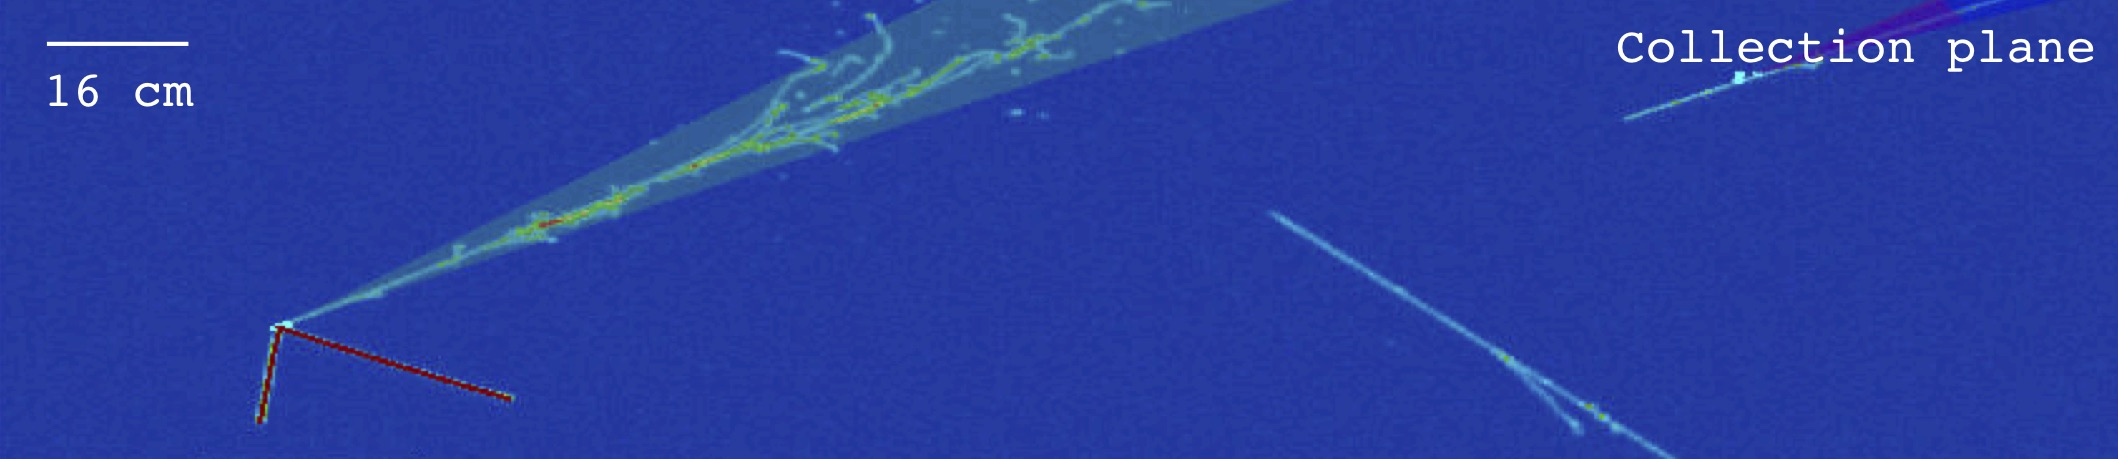
\includegraphics[width=0.8\linewidth]{figures/evd.jpg}
    	\caption{Monte Carlo event display of the collection plane with an electron and two protons in the final state. The reconstructed shower-like object is represented by the green cone. The reconstructed track-like objects are represented by the red lines.} \label{fig:evd}
	\end{center}
\end{figure}

Figure \ref{fig:anadia} shows a diagram of the three stages of the analysis paths.
Our $\nu_{e}$ CC0$\pi$-Np selection algorithm first looks for (1) a flash in the optical system compatible with the neutrino interaction, plus (2) a vertex in the TPC shared by  one or more track objects and one or more shower objects, or two or more shower objects. 
Then, the $\nu_{\mu}$ candidates selected by an external module \cite{ubxsec} are removed from the sample. The signal events are further isolated applying several boxed cuts on kinematic, geometric, and calorimetric variables, as described in Section \ref{sec:cuts}. Finally, the energy spectrum of the $\nu_{e}$ CC0$\pi$-Np candidates is measured with the procedure described in Section \ref{sec:energyreco}.

\begin{figure}[htbp]
\centering
\tikzset{every picture/.style={line width=0.75pt}} %set default line width to 0.75pt        
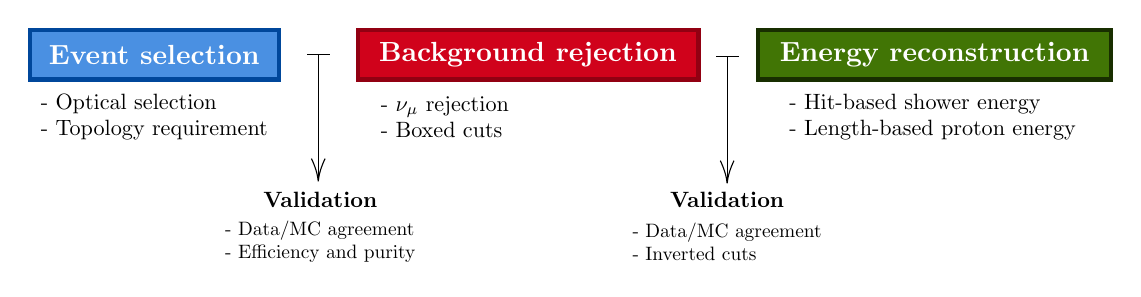
\begin{tikzpicture}[x=0.75pt,y=0.75pt,yscale=-1,xscale=1]
%uncomment if require: \path (0,163); %set diagram left start at 0, and has height of 163

\draw    (211,34) -- (211,95) ;
\draw [shift={(211,95)}, rotate = 270] [color={rgb, 255:red, 0; green, 0; blue, 0 }  ]   (0,0) .. controls (3.31,-0.3) and (6.95,-1.4) .. (10.93,-3.29)(0,0) .. controls (3.31,0.3) and (6.95,1.4) .. (10.93,3.29)   ;
\draw [shift={(211,34)}, rotate = 270] [color={rgb, 255:red, 0; green, 0; blue, 0 }  ]   (0,5.59) -- (0,-5.59)   ;
\draw    (408,35) -- (408,96) ;
\draw [shift={(408,96)}, rotate = 270] [color={rgb, 255:red, 0; green, 0; blue, 0 }  ]   (0,0) .. controls (3.31,-0.3) and (6.95,-1.4) .. (10.93,-3.29)(0,0) .. controls (3.31,0.3) and (6.95,1.4) .. (10.93,3.29)   ;
\draw [shift={(408,35)}, rotate = 270] [color={rgb, 255:red, 0; green, 0; blue, 0 }  ]   (0,5.59) -- (0,-5.59)   ;

\draw  [color={rgb, 255:red, 0; green, 71; blue, 155 }  ,draw opacity=1 ][fill={rgb, 255:red, 74; green, 144; blue, 226 }  ,fill opacity=1 ][line width=1.5]    (72, 22) rectangle (192.05, 46)   ;
\draw (132,34) node  [align=left] {\textbf{\textcolor[rgb]{1,1,1}{Event selection}}};
\draw (132,64) node [scale=0.8] [align=left] {
\mbox{-} Optical selection\\
\mbox{-} Topology requirement
};
\draw (212,104) node [scale=0.8] [align=left] {\textbf{Validation}};
\draw  [color={rgb, 255:red, 146; green, 0; blue, 18 }  ,draw opacity=1 ][fill={rgb, 255:red, 208; green, 2; blue, 27 }  ,fill opacity=1 ][line width=1.5]    (230, 22) rectangle (394.2, 46)   ;
\draw (312,34) node [color={rgb, 255:red, 255; green, 255; blue, 255 }  ,opacity=1 ] [align=left] {\textbf{Background rejection}};
\draw (272,64) node [scale=0.8] [align=left] {
\mbox{-} $\nu_{\mu}$ rejection\\
\mbox{-} Boxed cuts
};
\draw (408,104) node [scale=0.8] [align=left] {\textbf{Validation}};
\draw  [color={rgb, 255:red, 24; green, 46; blue, 0 }  ,draw opacity=1 ][fill={rgb, 255:red, 65; green, 117; blue, 5 }  ,fill opacity=1 ][line width=1.5]    (423, 22) rectangle (593.05, 46)   ;
\draw (508,34) node [color={rgb, 255:red, 255; green, 255; blue, 255 }  ,opacity=1 ] [align=left] {\textbf{Energy reconstruction}};
\draw (507,64) node [scale=0.8] [align=left] {
\mbox{-} Hit-based shower energy\\
\mbox{-} Length-based proton energy
};
\draw (212,124) node [scale=0.7] [align=left] {
\mbox{-} Data/MC agreement\\
\mbox{-} Efficiency and purity
};
\draw (408,124) node [scale=0.7] [align=left] {
\mbox{-} Data/MC agreement\\
\mbox{-} Inverted cuts
};
\end{tikzpicture}
\caption{Diagram describing the analysis path. It can be divided into three main stages: event selection, background rejection and energy reconstruction. }\label{fig:anadia}
\end{figure}

\subsection{Optical selection}

The first requirement ensures the presence of light in the detector in a position compatible with the center of the collected charge of the neutrino interaction candidate and with a timing compatible with the beam-gate window.

It is also possible and likely that an event will have multiple neutrino candidates. The goal of the optical selection is reducing the number of candidates to maximal one candidate in each event. This process consists of three major parts:
\begin{enumerate}
\item Rectangular cuts are applied to optical properties of the reconstructed flash object.
\item Rectangular cuts on the compatibility of the reconstructed flash with the Pandora neutrino candidate.
\item The Pandora neutrino candidate which is most compatible with the flash is picked using a likelihood method.
\end{enumerate}

To demonstrate the effect of the used cuts, they will be applied on two different samples, both of which were produced with Monte Carlo Challenge 8.3:
\begin{itemize}
\item The signal sample: BNB $\nu_e$ intrinsic with cosmic rays
\begin{itemize}
\item The truth vertex should be in the fiducial volume.
\item There should be an electron with a kinetic energy of at least \SI{20}{\MeV}.
\item There should be at least one proton wit a kinetic energy of \SI{40}{\MeV} or higher.
\end{itemize}
\item The background sample: CORSIKA in-time cosmic rays
\end{itemize}

\begin{figure}[!htbp]
\centering
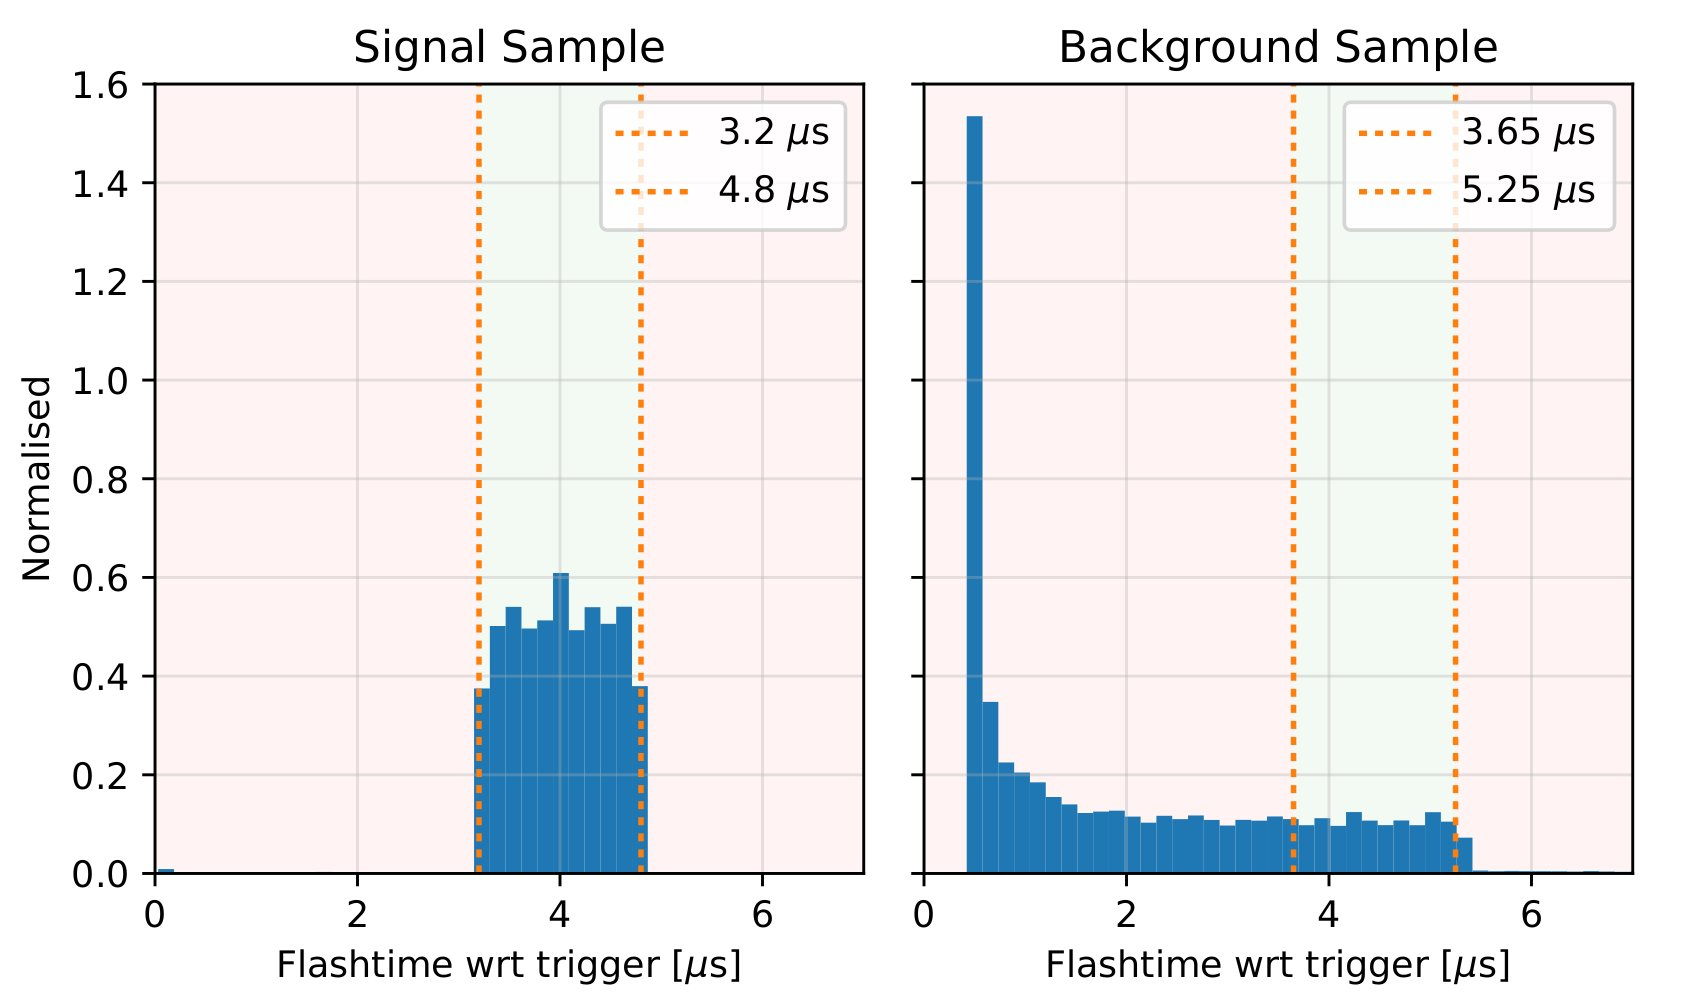
\includegraphics[width=0.75\textwidth]{beam}
\caption{Requirement a reconstructed flash object within the beam spill time window.} 
\label{fig:beam}
\end{figure}

The first requirement is that there is a reconstructed flash within the beam spill window of \SI{1.6}{\micro\s}. This cut is shown in Figure~\ref{fig:beam}. 99.6\% in the signal sample passes, 18.5\% in the background sample passes.

\begin{figure}[htbp]
\centering
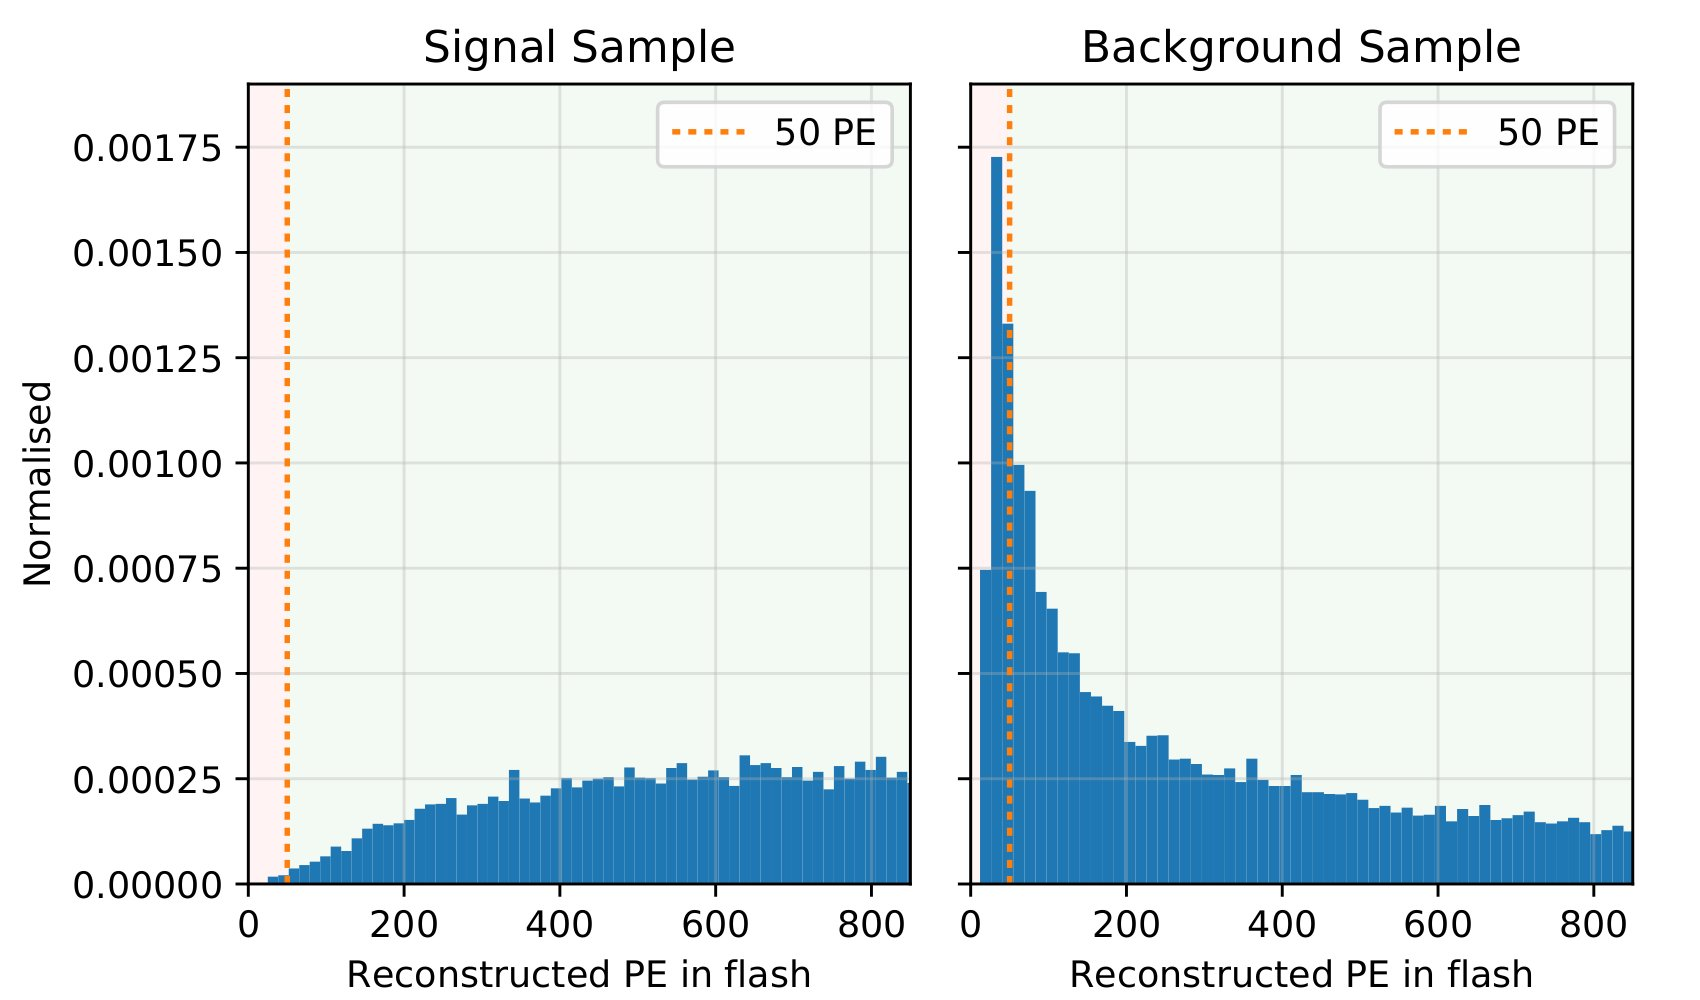
\includegraphics[width=0.75\textwidth]{PE}
\caption{Intensity of the reconstructed flash in photo-electrons. A cut is placed at 50 PE.} 
\label{fig:PE}
\end{figure}

After that, the reconstructed flash is required to consist of at least 50 photo-electrons (PE). This is a very conservative cut and keeps 99.95\% of the signal while 95.2\% of the background passes too. The PE distributions are given in Figure~\ref{fig:PE}.

\begin{figure}[htbp]
\centering
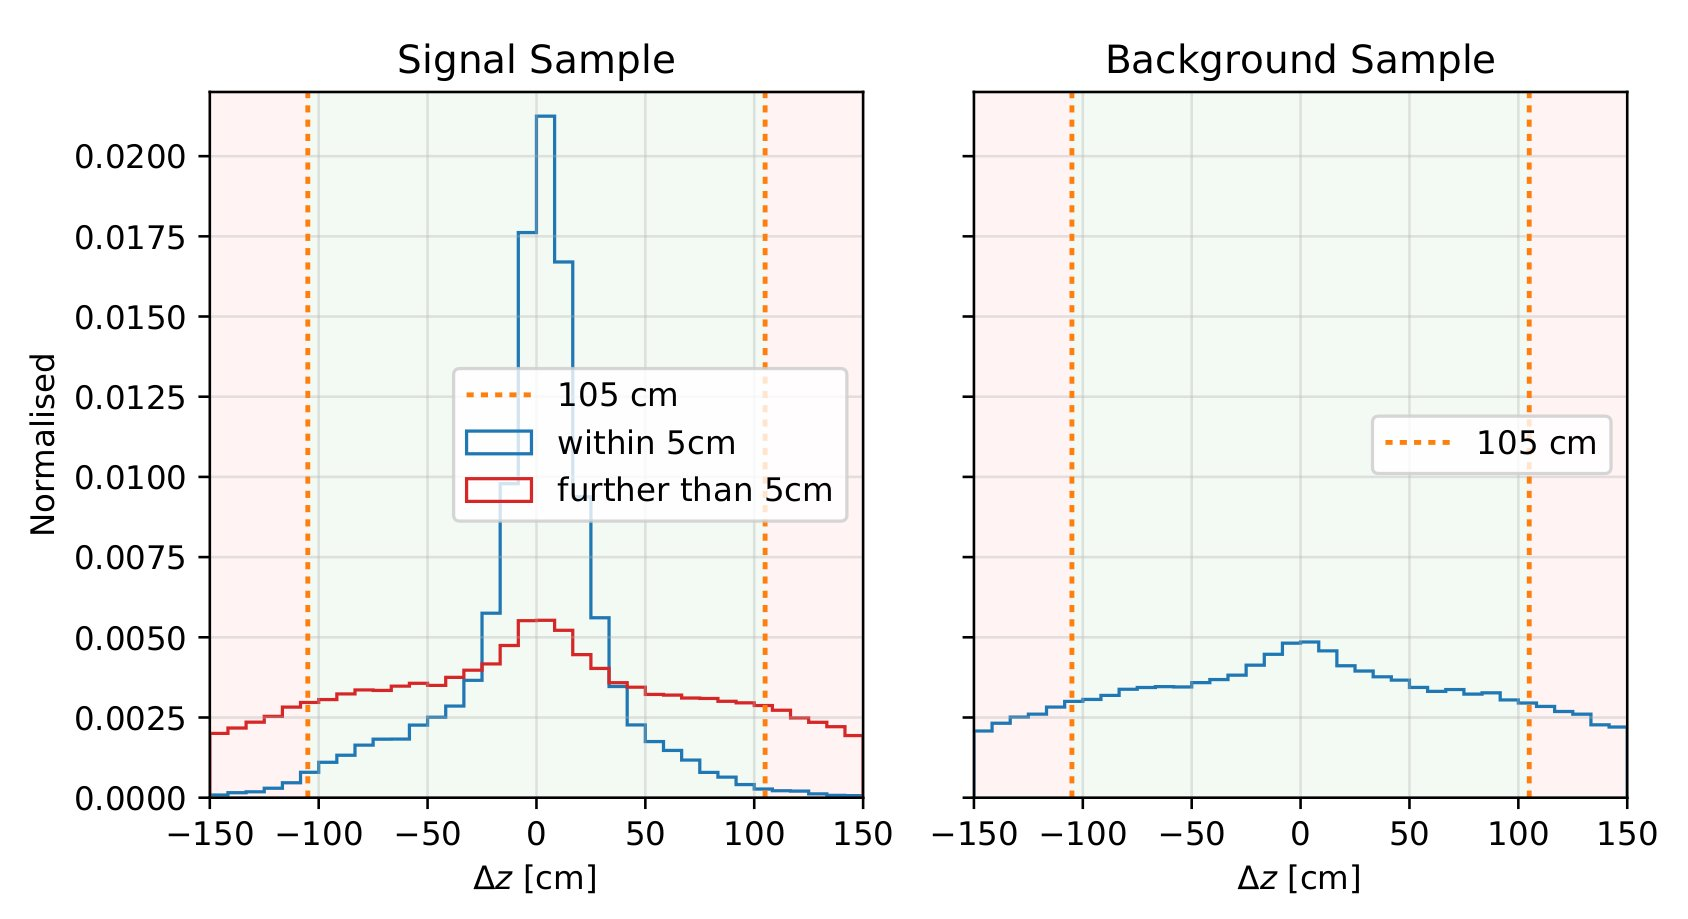
\includegraphics[width=0.8\textwidth]{zcut}
\caption{The distance between the flash and centre of deposited charge of the Pandora neutrino candidate. It is required that this is less than \SI{105}{\cm}.} 
\label{fig:zcut}
\end{figure}

At this point it is guaranteed that the event has a properly reconstructed flash. A flash object has a time and a PE count for each of the 32 PMT's. From that, a position $Z\pm \sigma_Z$ and $Y\pm \sigma_Y$ are calculated. These can be compared with the. centre of deposited charge of the Pandora candidate. This comparison has the implicit assumption that the light will be emitted in the same relative fraction as the charge is deposited by the final state particles. This is not completely correct since the amount of scintillation light produced per deposited \SI{1}{\MeV} is particle dependent. Nevertheless, compared to the coarse resolution of the PMT grid, this approximation is justified. In Figure~\ref{fig:zcut}, The effect of this cut is demonstrated. The signal sample is split up in two categories using truth information. Pandora neutrino candidates with their reconstructed vertex within \SI{5}{\cm} from the true vertex, and Pandora neutrino candidates with their reconstructed vertex further away. Those candidates with a misreconstructed vertex are often related to cosmic interaction, either mixed with neutrino activity or pure background. We therefore expect this group in the signal sample to follow the distribution of the background sample, which is confirmed in the figure. A cut is placed on a difference of \SI{105}{\cm} difference between the reconstructed flash position and the position of the deposited charge. This cut keeps at least one neutrino candidate in 98.1\% of the signal while it removes all neutrino candidates in 20\% of the background event. 
Similar cuts are obtained taking into account the width of the flash and the $y$-position. 

\begin{figure}[!htbp]
\centering
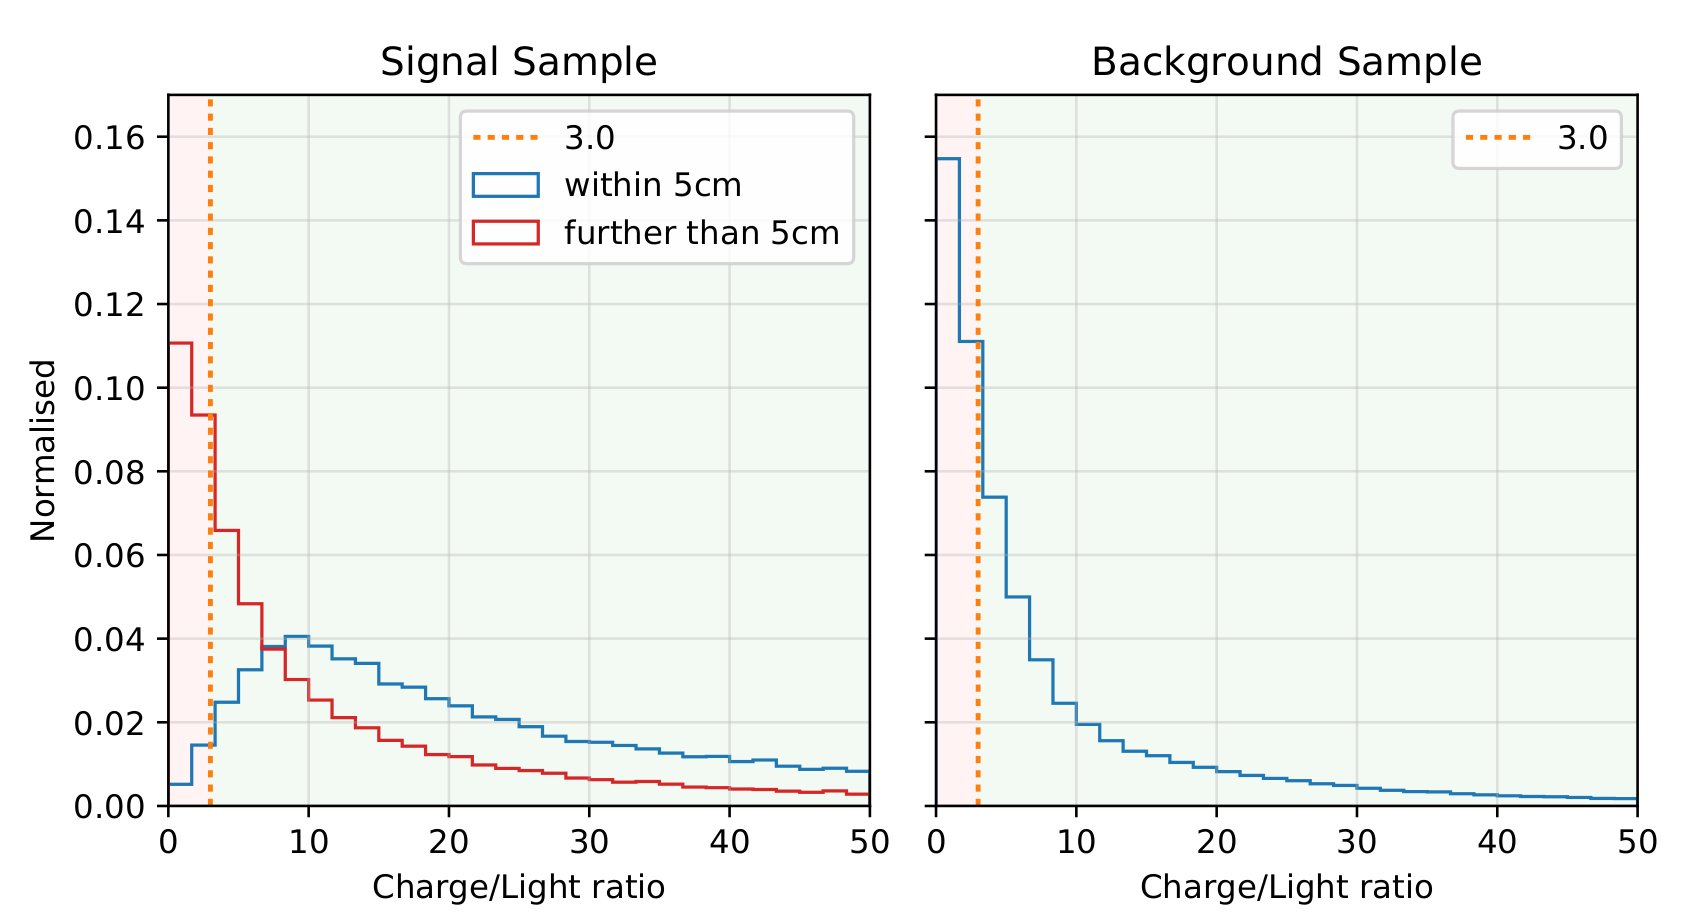
\includegraphics[width=0.8\textwidth]{charge}
\caption{For neutrino interactions, the a higher amount of deposited charge will come together with a more intense reconstructed flash. A cut on the ratio of higher than 3.0 is imposed on the neutrino candidates.} 
\label{fig:charge}
\end{figure}

The last rectangular cut exploits the fact that a lot of the neutrino candidates reconstructed by Pandora originate from remainders of cosmic activity that was not completely removed in the cosmic removal stage of the reconstruction. Those neutrino candidates often consist of a small amount of fragmented charge, incompatible with the brightness of the flash. In Figure~\ref{fig:charge}, the ratio of deposited charge associated to a neutrino candidate and the  amount of photo-electrons in the reconstructed flash is shown. The signal sample is again split up in two categories as before. Placing a very conservative cut at 3.0 reduces the signal events with a properly reconstructed flash with 1.7\% while removing all neutrino candidates in 15.4\% of the events. 

\begin{figure}[!htbp]
\centering
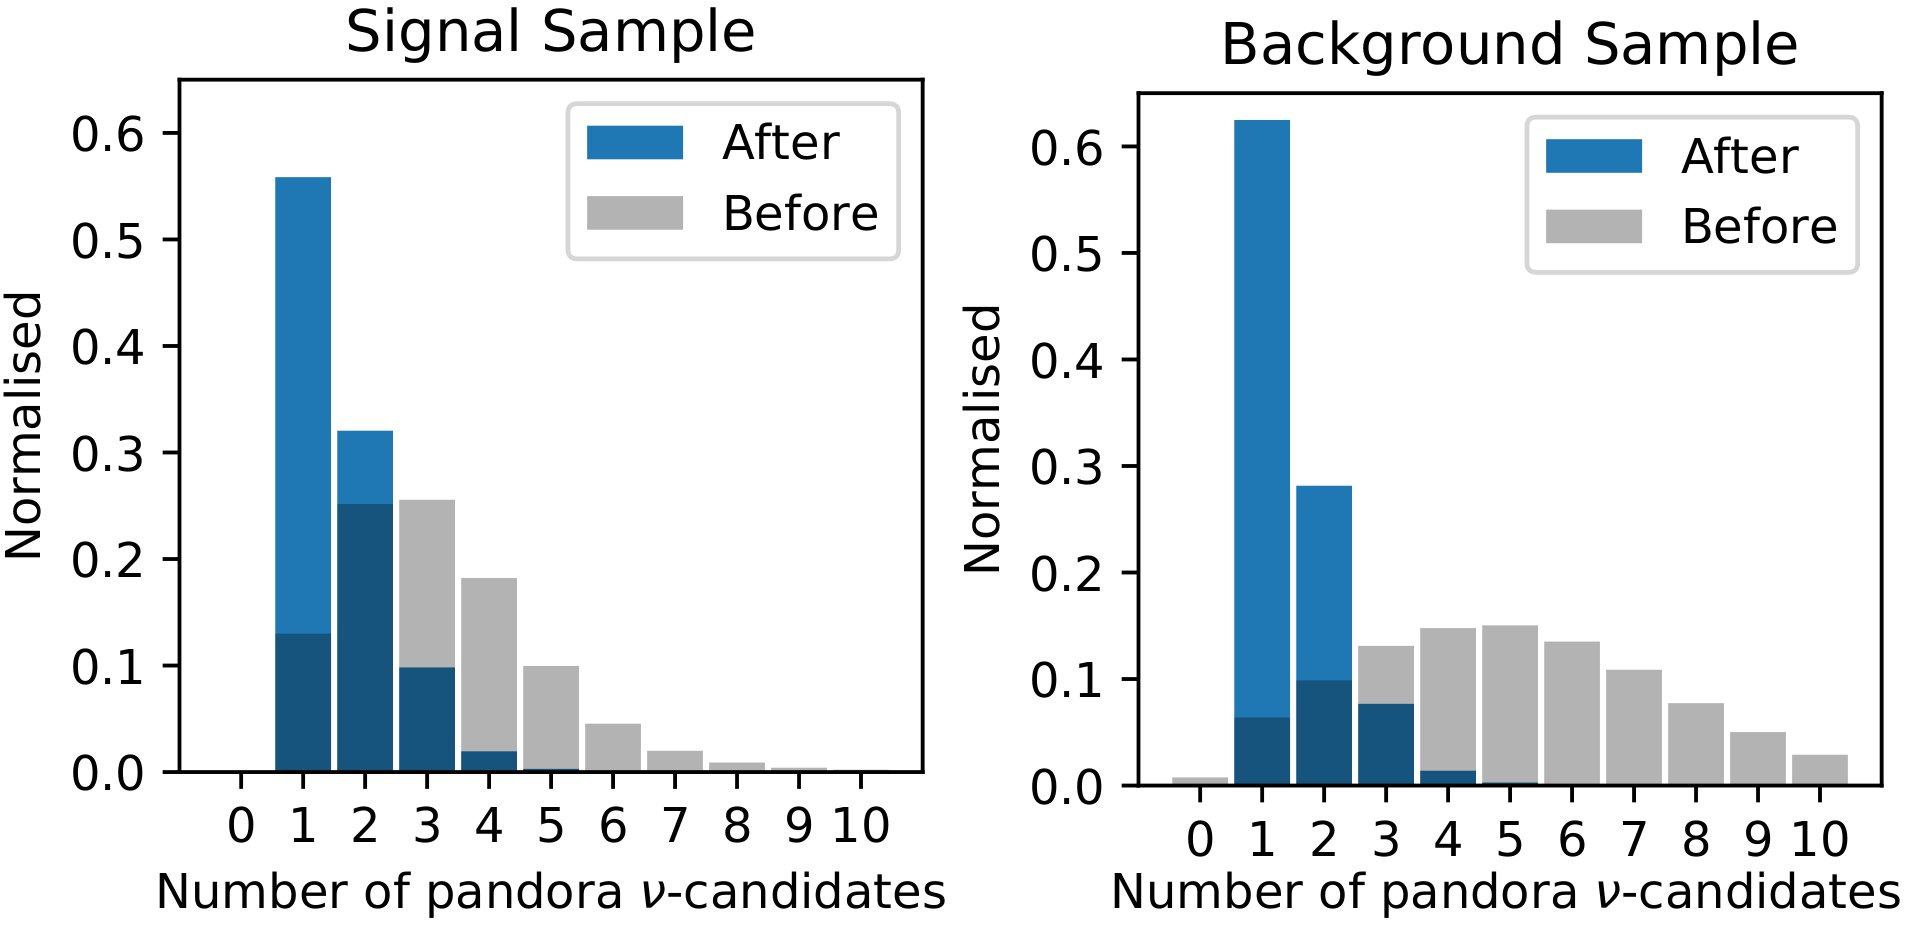
\includegraphics[width=0.8\textwidth]{boxed}
\caption{Effect of the rectangular optical cuts on the amount of Pandora neutrino candidates .} 
\label{fig:boxed}
\end{figure}

After applying the two sets of described rectangular cuts. It is informative to not only discuss the passing rates, but also the number of neutrino candidates remaining in the passed events. This is shown in Figure~\ref{fig:boxed}. In Grey, the number of neutrino candidates before any cuts is shown. In blue, the number of candidates that passed the rectangular cuts is shown. In about half of the remaining cases, there are multiple neutrino candidates remaining, this will be reduced to exactly one per passing event using flash-matching. 

\begin{figure}[!htbp]
\centering
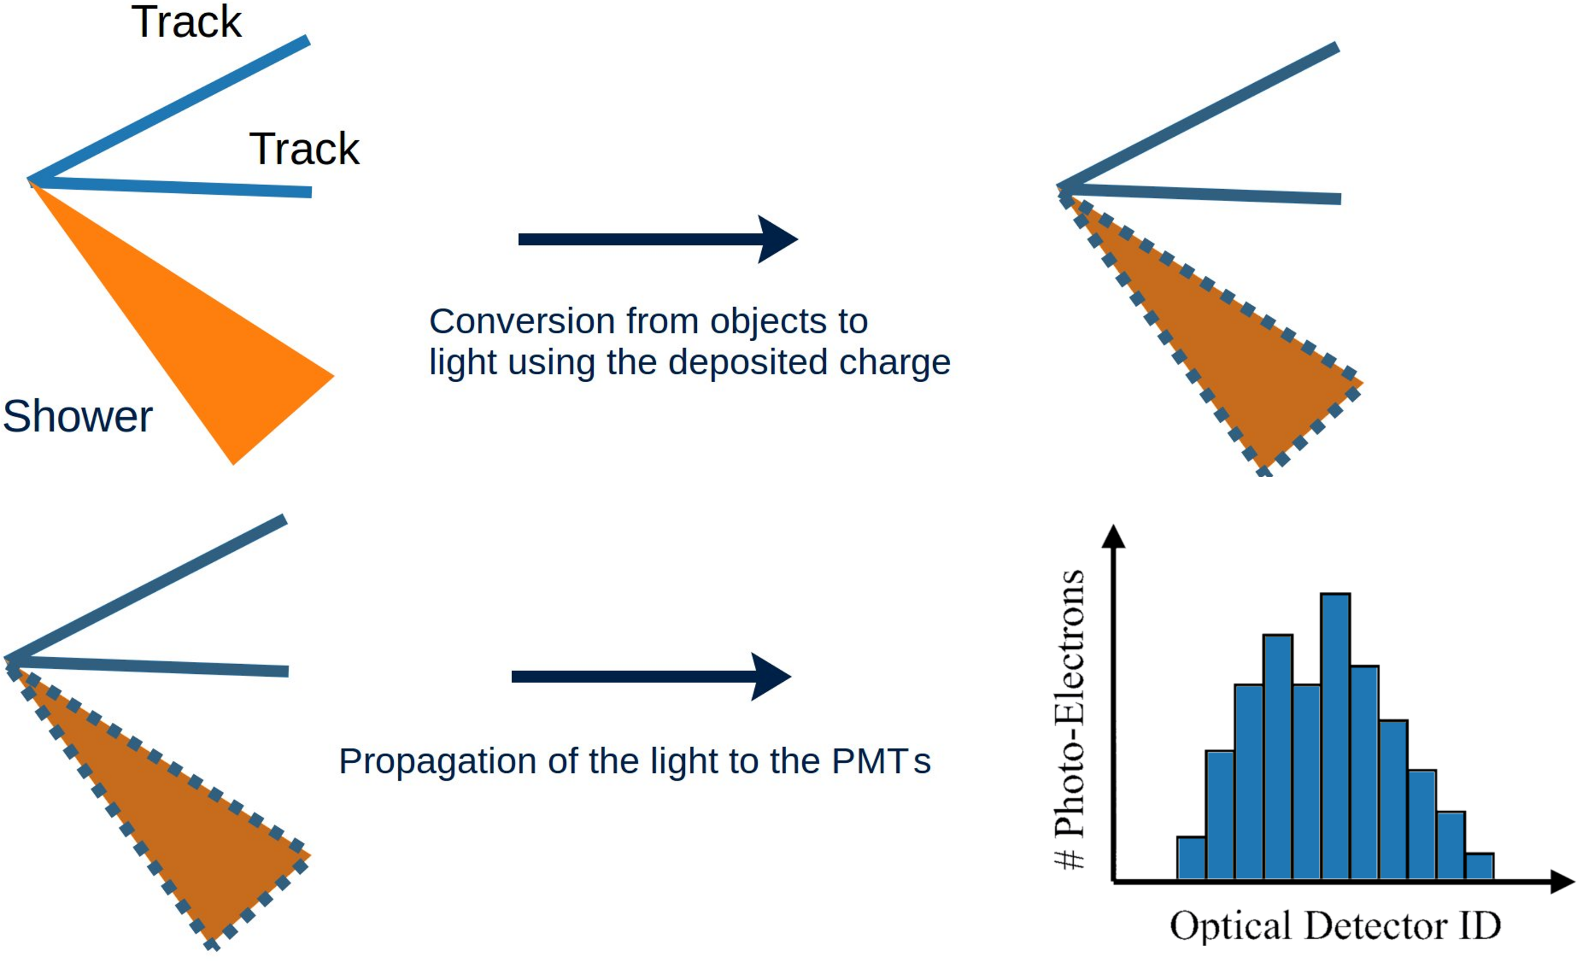
\includegraphics[width=0.7\textwidth]{flashdrawing} 
\caption{Schematic of the construction of a flash hypothesis for a neutrino candidate.} 
\label{fig:flashdrawing}
\end{figure}

The principle of flash-matching is described in Figure~\ref{fig:flashdrawing}:
\begin{itemize}
\item A flash hypothesis can be constructed for each candidate vertex using only data recorded by the time projection chamber.
\item For every neutrino candidate, a spatial distribution of deposited charge can be constructed.
\item The spatial distribution of the deposited charge is translated into an estimation of the emitted scintillation light. These scintillation photons are then propagated towards the PMTs to construct a flash hypothesis using only time projection chamber information.
\item The flash-matching algorithm compares the reconstructed flash object as seen by the PMT's with the hypothetical flash for all possible neutrino candidates and picks the best matching candidate. For this, a binned likelihood of the PMT spectrum is optimised.
\end{itemize}
An example of this procedure for a Monte Carlo generated $\nu_e$ event with 4 neutrino candidates is given in Figure~\ref{fig:flashmatch}.
\begin{figure}[!htbp]
\centering
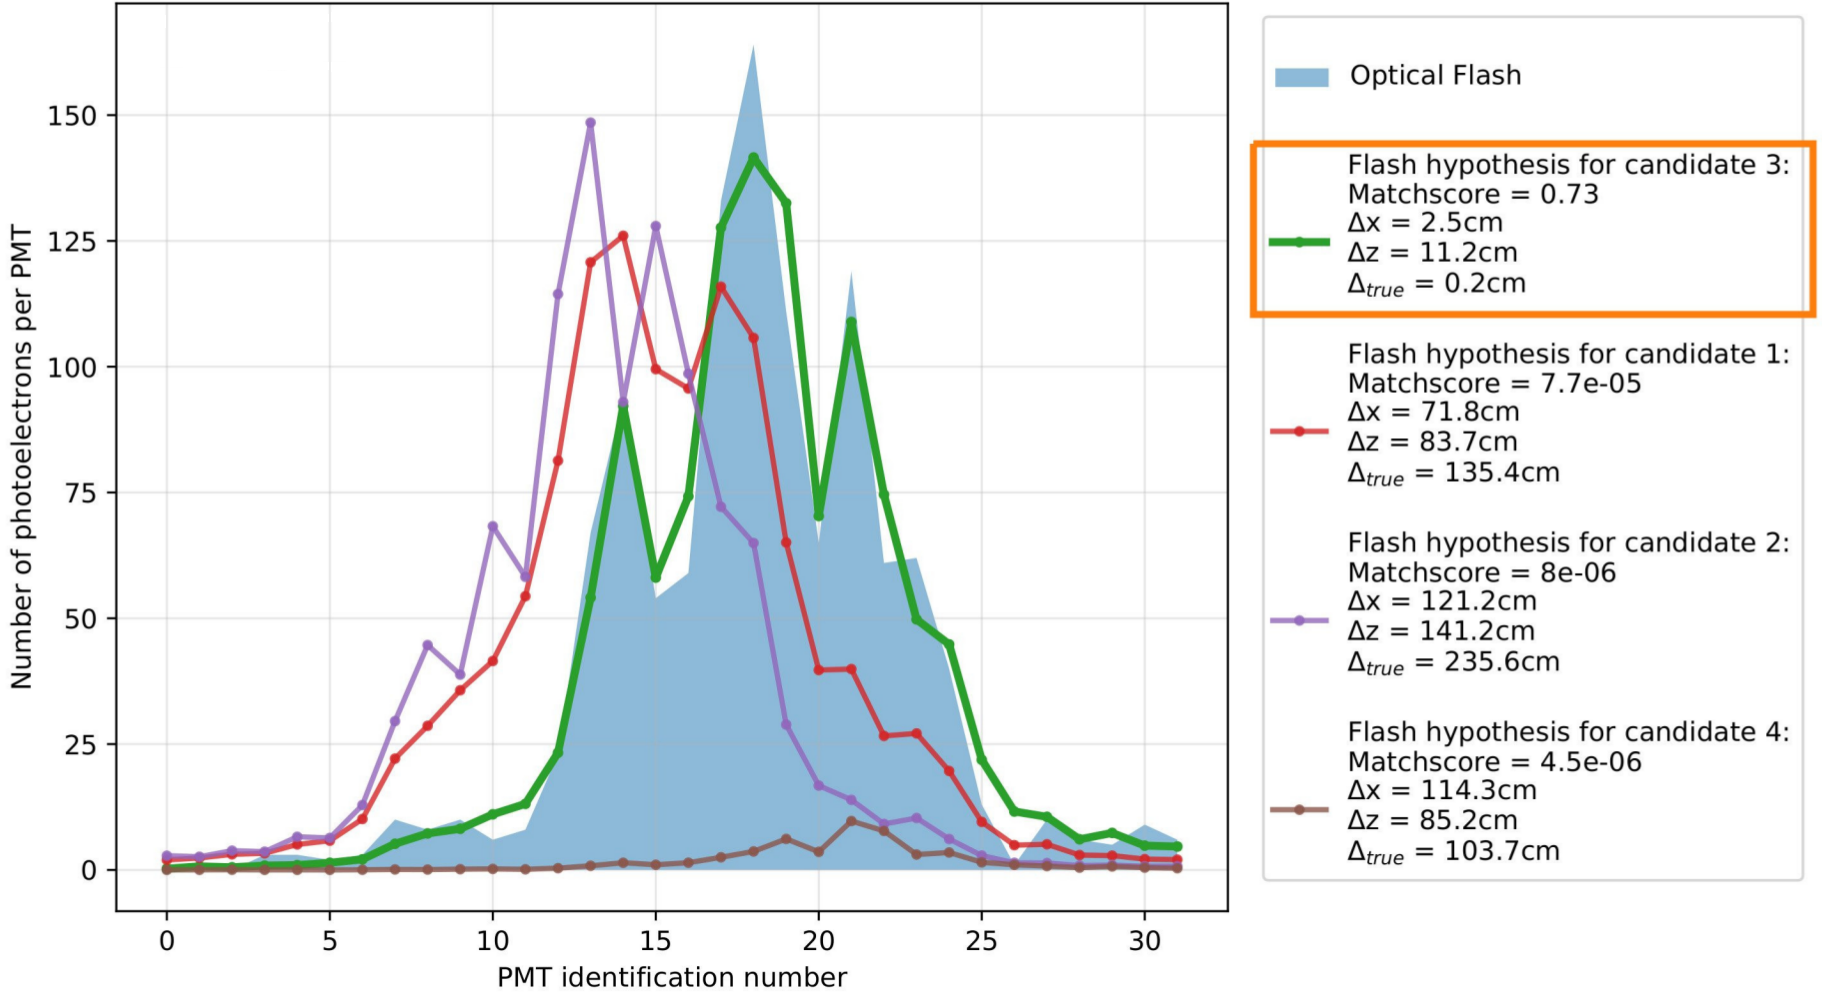
\includegraphics[width=0.85\textwidth]{flashmatch} 
\caption{An example of flash-matching. Event with 4 neutrino candidates, for all of the candidates the flash hypothesis is constructed and matched to the reconstructed flash (shaded blue). For all candidates a minimum binned likelihood is calculated, varying the $x$ position of the interaction. The match score is the inverse of the likelihood. For all neutrino candidates, the reconstructed vertex is compared with the true distance and given by $\Delta_{true}$ } 
\label{fig:flashmatch}
\end{figure}

\subsection{Topology requirement}
A perfect reconstruction of a $\nu_{e}$ CC0$\pi$-Np event in a LArTPC will produce as many reconstructed tracks as the number of protons in the final state and a single reconstructed shower (the electron), sharing a common vertex. However, the presence of missing or unresponsive wires can cause the splitting of an ionisation track or an electromagnetic showers into two distinct reconstructed object. Also, the type of object (track or shower) is assigned by a Support Vector Machine implemented in the Pandora framework and its performances depend on the quality of the event (e.g. the number of hits). A track-like object (e.g. a proton or a muon), then, can be mis-reconstructed as a shower object, especially when the number of reconstructed hits is low \cite{pandora2}. In order to maximise our efficiency, then, we will require (1) \emph{at least} one track and \emph{at least} one shower sharing a common vertex, or (2) \emph{at least} two showers sharing a common vertex. Figure \ref{fig:dia} shows the two diagrams of the accepted topologies for a $\nu_{e}$ CC0$\pi$-Np candidate event.

\begin{figure}
\centering
  \begin{subfigure}{0.4\textwidth}
    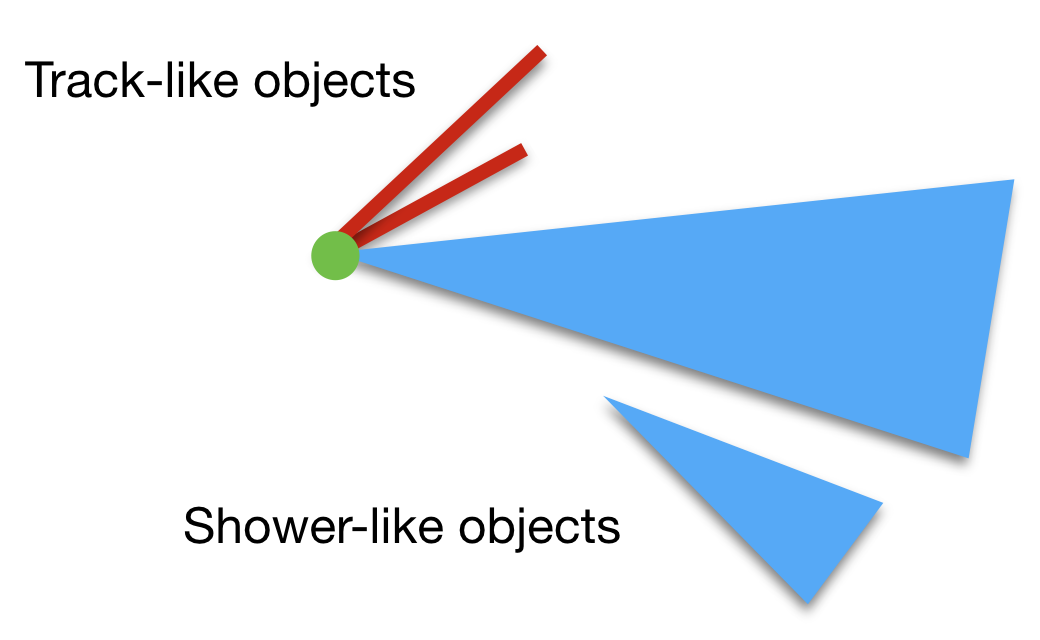
\includegraphics[width=\linewidth]{figures/trsh.png}
    \caption{1+ tracks and 1+ showers} 
  \end{subfigure}
    \begin{subfigure}{0.4\textwidth}
    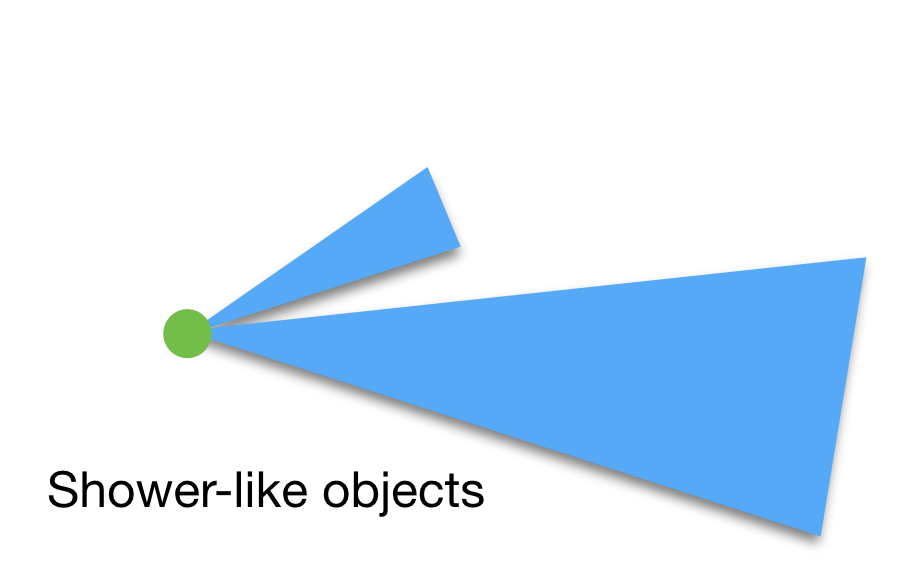
\includegraphics[width=\linewidth]{figures/sh.png}
    \caption{2+ showers} 
  \end{subfigure}
  \caption{The selection algorithm requires a neutrino candidate with one or more tracks and one or more shower sharing (left) or two or more showers (right) sharing  a common vertex.}\label{fig:dia}
\end{figure}

Figure \ref{fig:2showers} shows a Monte Carlo event display with an electromagnetic shower correctly reconstructed as a shower-like object and a proton track mis-reconstructed as a shower-like object. Requiring at least two showers allows to recover this kind of event.

\begin{figure}[htbp]
	\begin{center}
    	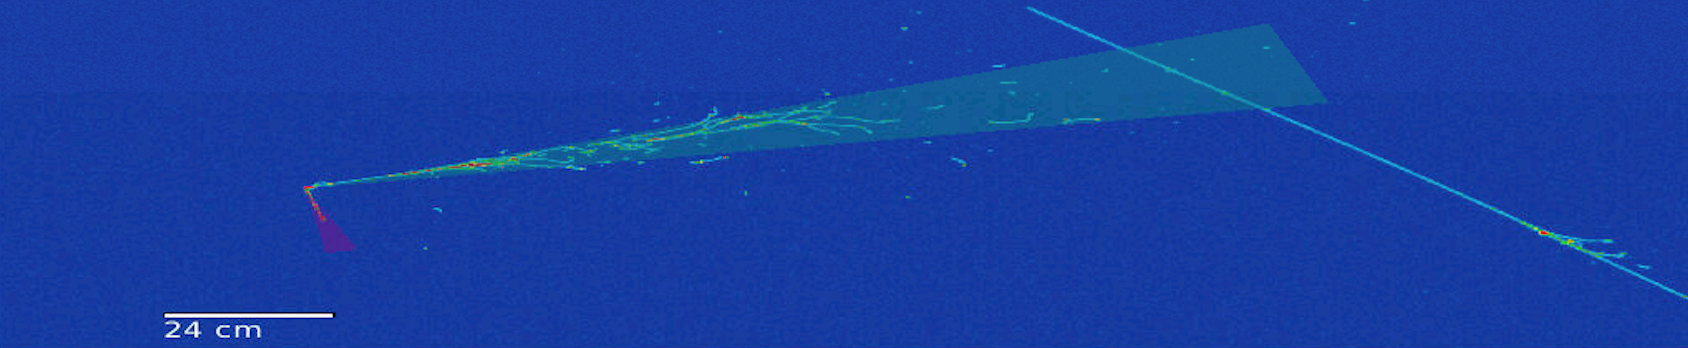
\includegraphics[width=0.8\linewidth]{figures/2showers.png}
    	\caption{Monte Carlo event display of the collection plane with one electron and one proton in the final state. The proton track has been mis-reconstructed as a shower-like object.} \label{fig:2showers}
	\end{center}
\end{figure}

In these cases, in order to choose the proton track candidate among the two shower-like objects, we run a bi-dimensional Principal Component Analysis in the collection plane (one dimension is given by the drift time and the other by the wire coordinate). The object with the largest first eigenvalue is chosen as the proton track candidate and it is then consider as a track-like object.

\subsection{Selection efficiency and purity}
In order to obtain a first estimate of the number of events that can be selected by our algorithm, we performed a study of the selection efficiency and purity using a dedicated $\nu_{e}$ CC$0\pi$-Np Monte Carlo sample. Neutrino events have been generated using the GENIE Neutrino Monte Carlo generator \cite{genie} and cosmic rays have been generated using the CORSIKA Monte Carlo generator \cite{corsika}. 

In this sample, every event has one $\nu_{e}$ interaction with one electron, at least one proton and no other visible particles in the final state (it can have neutrons). 

In order to avoid border effects, such as electric field non-uniformities, the true neutrino interaction vertex must lie within a fiducial volume. Our fiducial volume cut is $\pm10$~cm on the $x$ axis, $\pm20$~cm on the $y$ axis, and $^{+10}_{-50}$~cm on the $z$ axis. 
Since electromagnetic showers develop mainly in the forward direction with respect to the beam, the asymmetric cut on the $z$ axis (which corresponds to the beam direction) helps reject non-fully contained events.

A study on the reconstruction efficiency of proton tracks and electron showers in $\nu_{e}$ CC$0\pi$-Np events shows that the efficiency is zero for proton with a kinetic energy below 40~MeV and for electrons with a kinetic energy below 20~MeV. As such, in our sample each event must have at least one proton above 40~MeV and one electron above 20~MeV. Figure \ref{fig:kin_eff} shows the reconstruction efficiencies for protons and electrons as a function of the kinetic energy.

\begin{figure}[htbp]
  \begin{subfigure}{0.48\textwidth}
    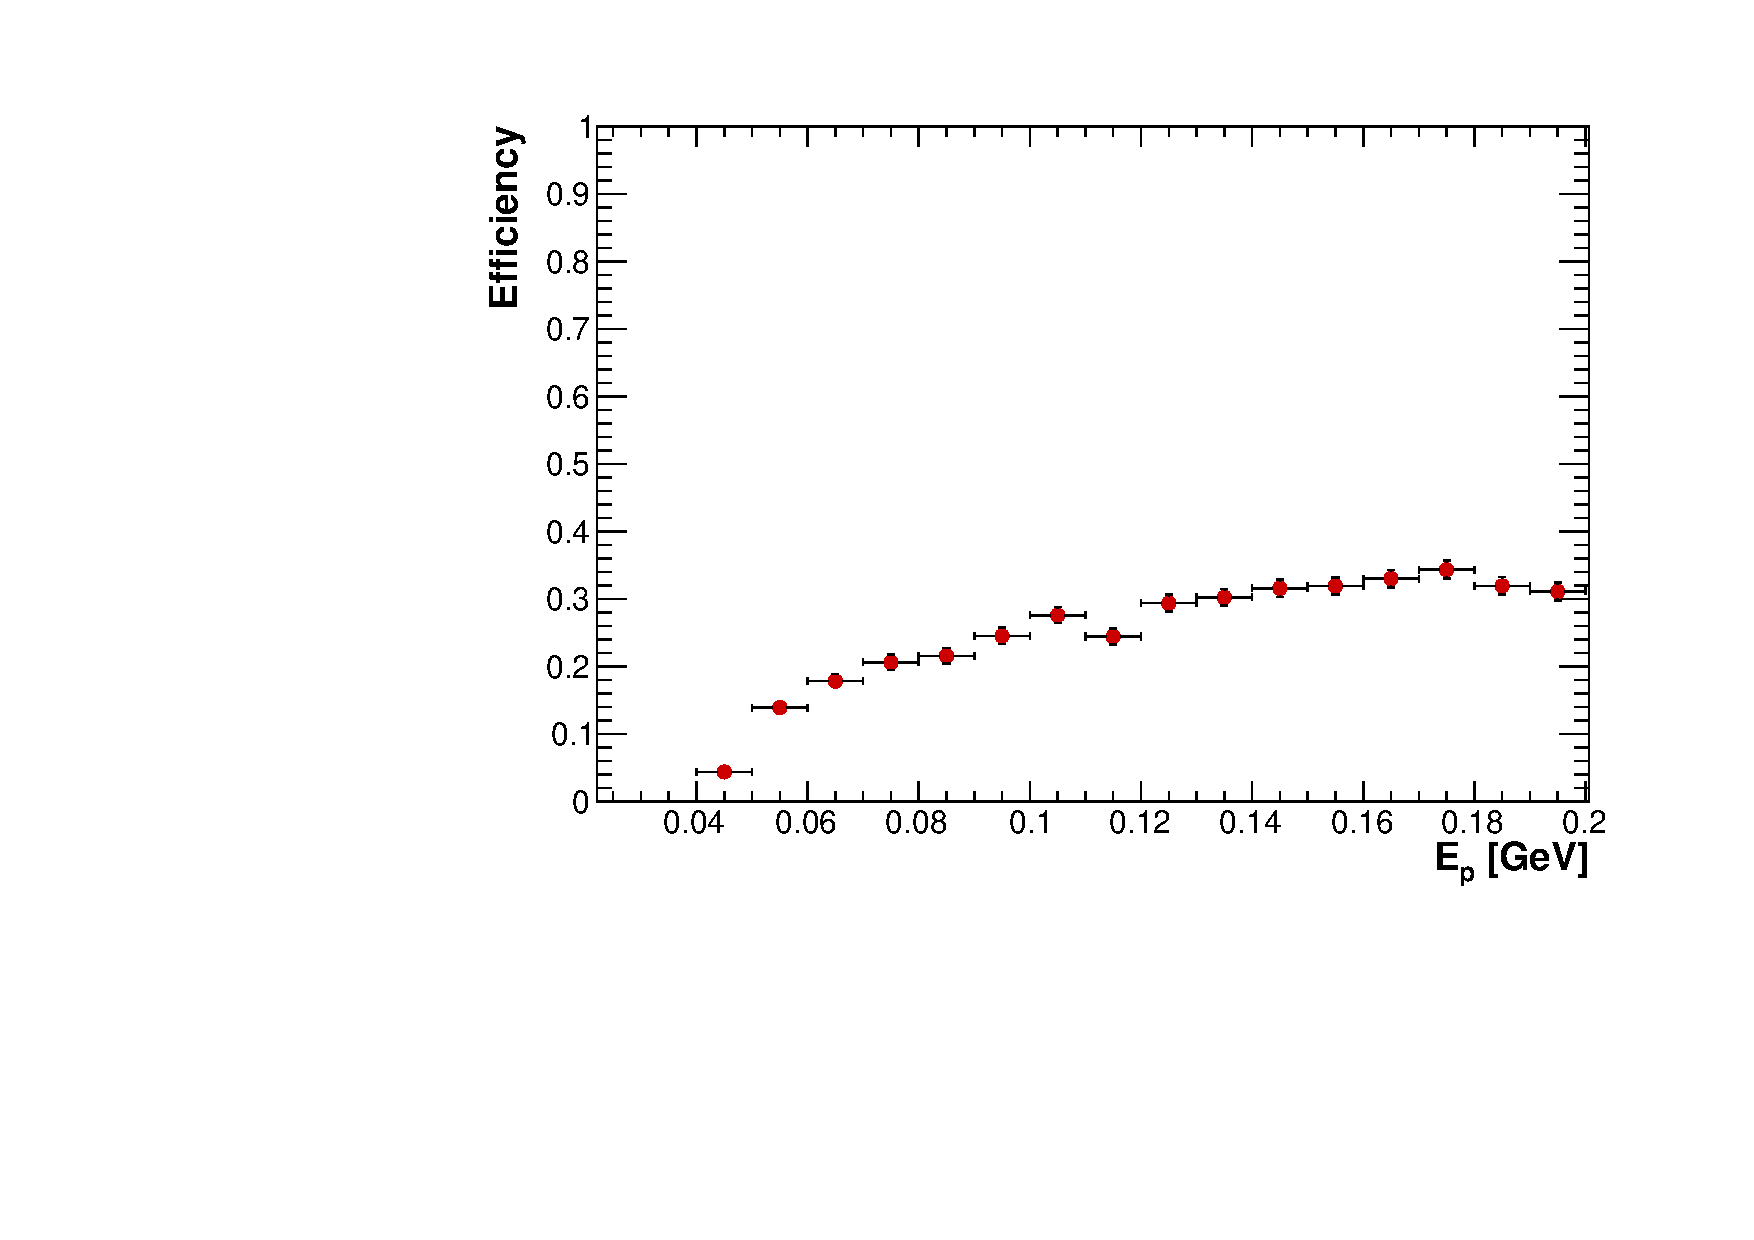
\includegraphics[width=\linewidth]{figures/proton_eff.pdf}
    \caption{Proton reconstruction efficiency} 
  \end{subfigure}
    \begin{subfigure}{0.48\textwidth}
    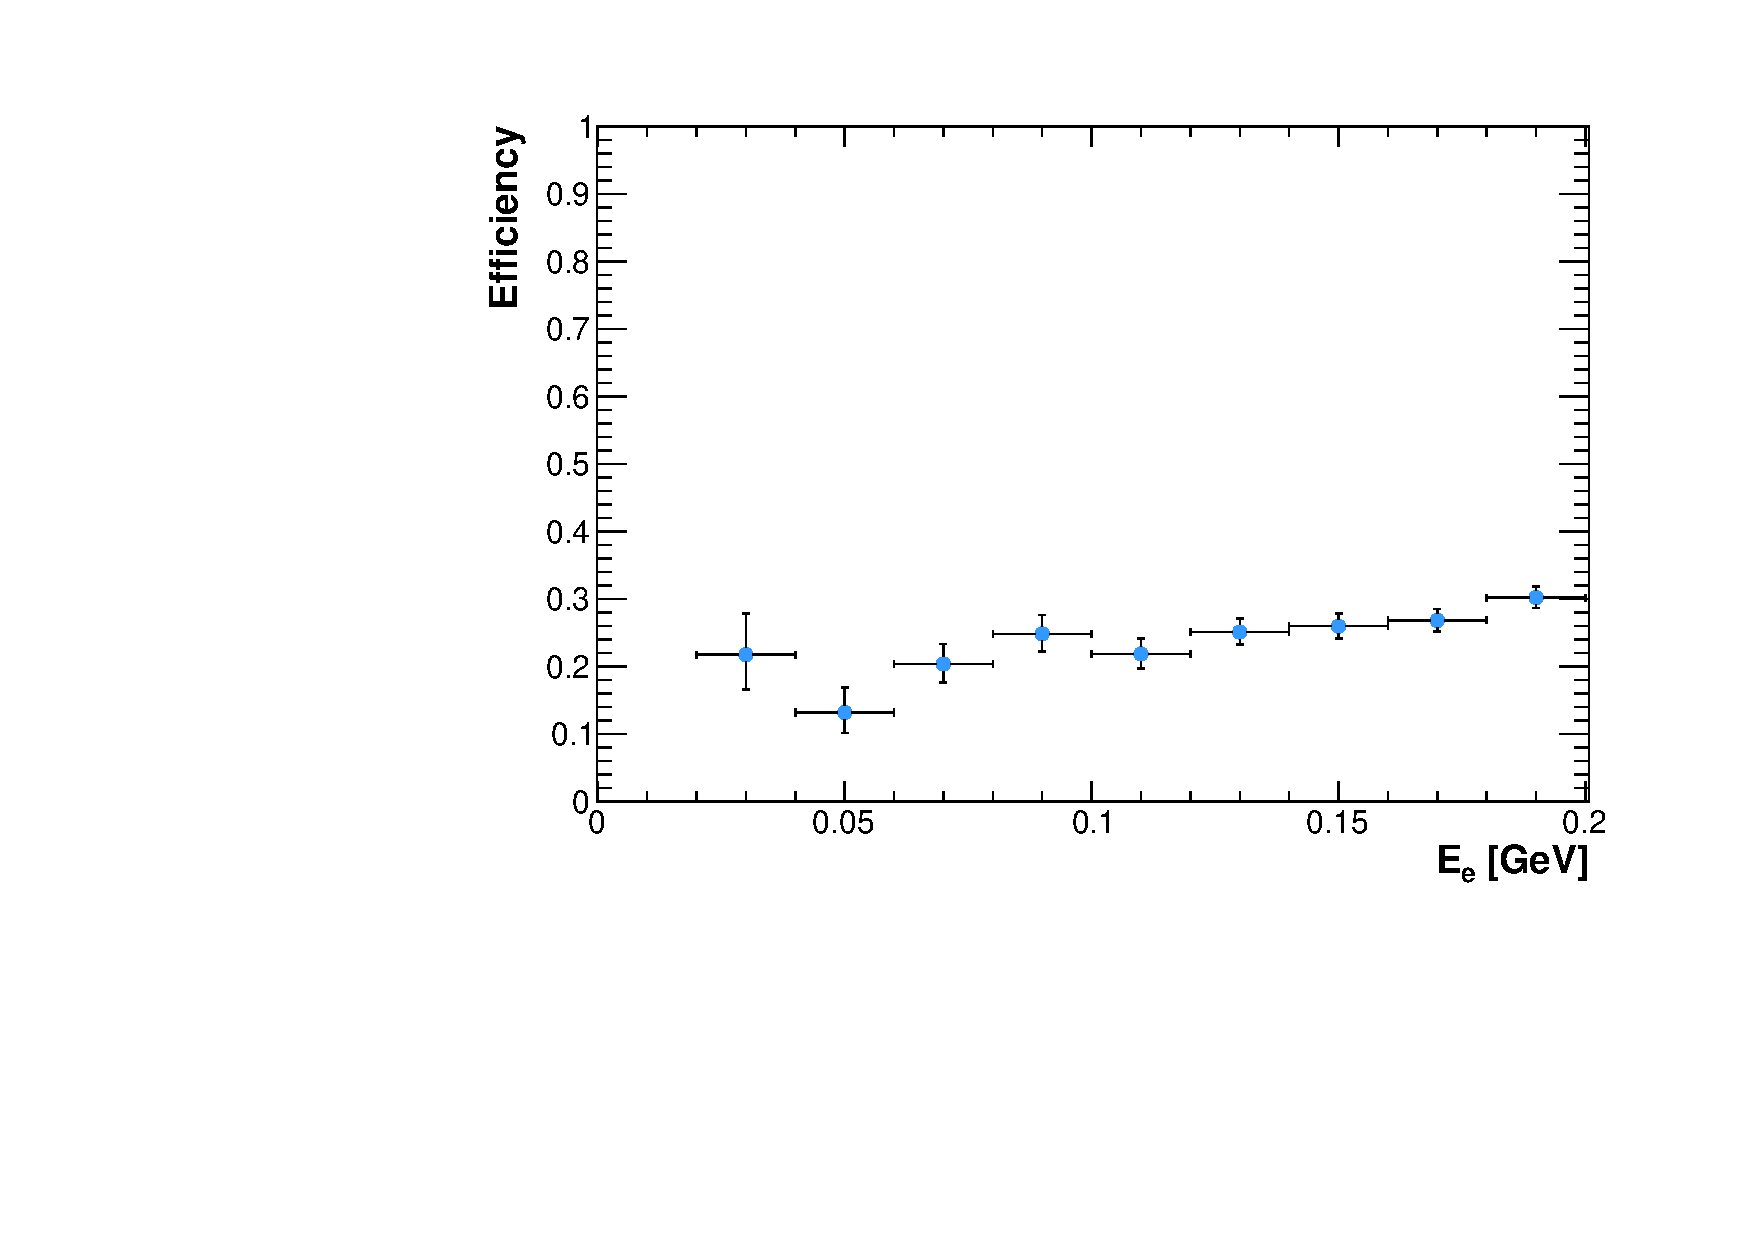
\includegraphics[width=\linewidth]{figures/electron_eff.pdf}
    \caption{Electron reconstruction efficiency} 
  \end{subfigure}
  \caption{Proton (left, in red) and electron (right, in blue) reconstruction efficiency for simulated $\nu_{e}$ CC$0\pi$-Np events. In our sample of generated $\nu_{e}$ CC$0\pi$-Np events we require at least a proton above 40~MeV and at least an electron above 20~MeV.}
  \label{fig:kin_eff}
\end{figure}


The selection efficiency $\epsilon$ is defined as:
\begin{equation}
\epsilon = \frac{\mathrm{N.~of~selected~CC0}\pi\mathrm{{\text -}Np~events}}{\mathrm{N.~of~generated~CC0}\pi\mathrm{{\text -}Np~events}},
\end{equation}
where each selected event must pass the optical selection, satisfy the topology requirement A minimum quality of the selected event is also ensured requiring (1) at least 5 hits in the collection plane associated to a shower-like object, (2) at least 5 hits in the collection plane associated to a track-like object, and (3) at least one hit in every wire.
The start and end point of each track-like object and the start point of each shower-like object must also lie within the fiducial volume to ensure that the event is fully contained.

The purity of the sample is defined as:
\begin{equation}
\epsilon = \frac{\mathrm{N.~of~selected~CC0}\pi\mathrm{{\text -}Np~events}}{\mathrm{N.~of~selected~events}},
\end{equation}
and it has been measured running the selection algorithm on a complete sample of neutrino events (not only $\nu_{e}$ interactions), weighted accordingly to the Booster Neutrino Beam (BNB) flux. In this sample every event will have at least one neutrino interacting in the cryostat volume and triggering the detector, plus all the cosmic rays hitting the detector in the same readout window. In the data, however, this is not always true, since the detector can be triggered also by a cosmic ray producing a flash in the optical system during the beam window, without necessarily having a neutrino interaction. In order to estimate this background component, defined as \emph{in-time cosmic rays}, we have used the data EXT sample, which was collected using the standard detector trigger, but with the neutrino beam off.

Figure \ref{fig:effpurity} shows the efficiency as a function of the true neutrino energy and the purity as a function of the reconstructed energy. The energy reconstruction procedure is described in section \ref{sec:energyreco}.
As expected, the efficiency (purity) is proportional to the neutrino energy (reconstructed energy), since high-energy events correspond in general to a larger number of hits in the TPC. 

\begin{figure}
  \begin{subfigure}{0.48\textwidth}
    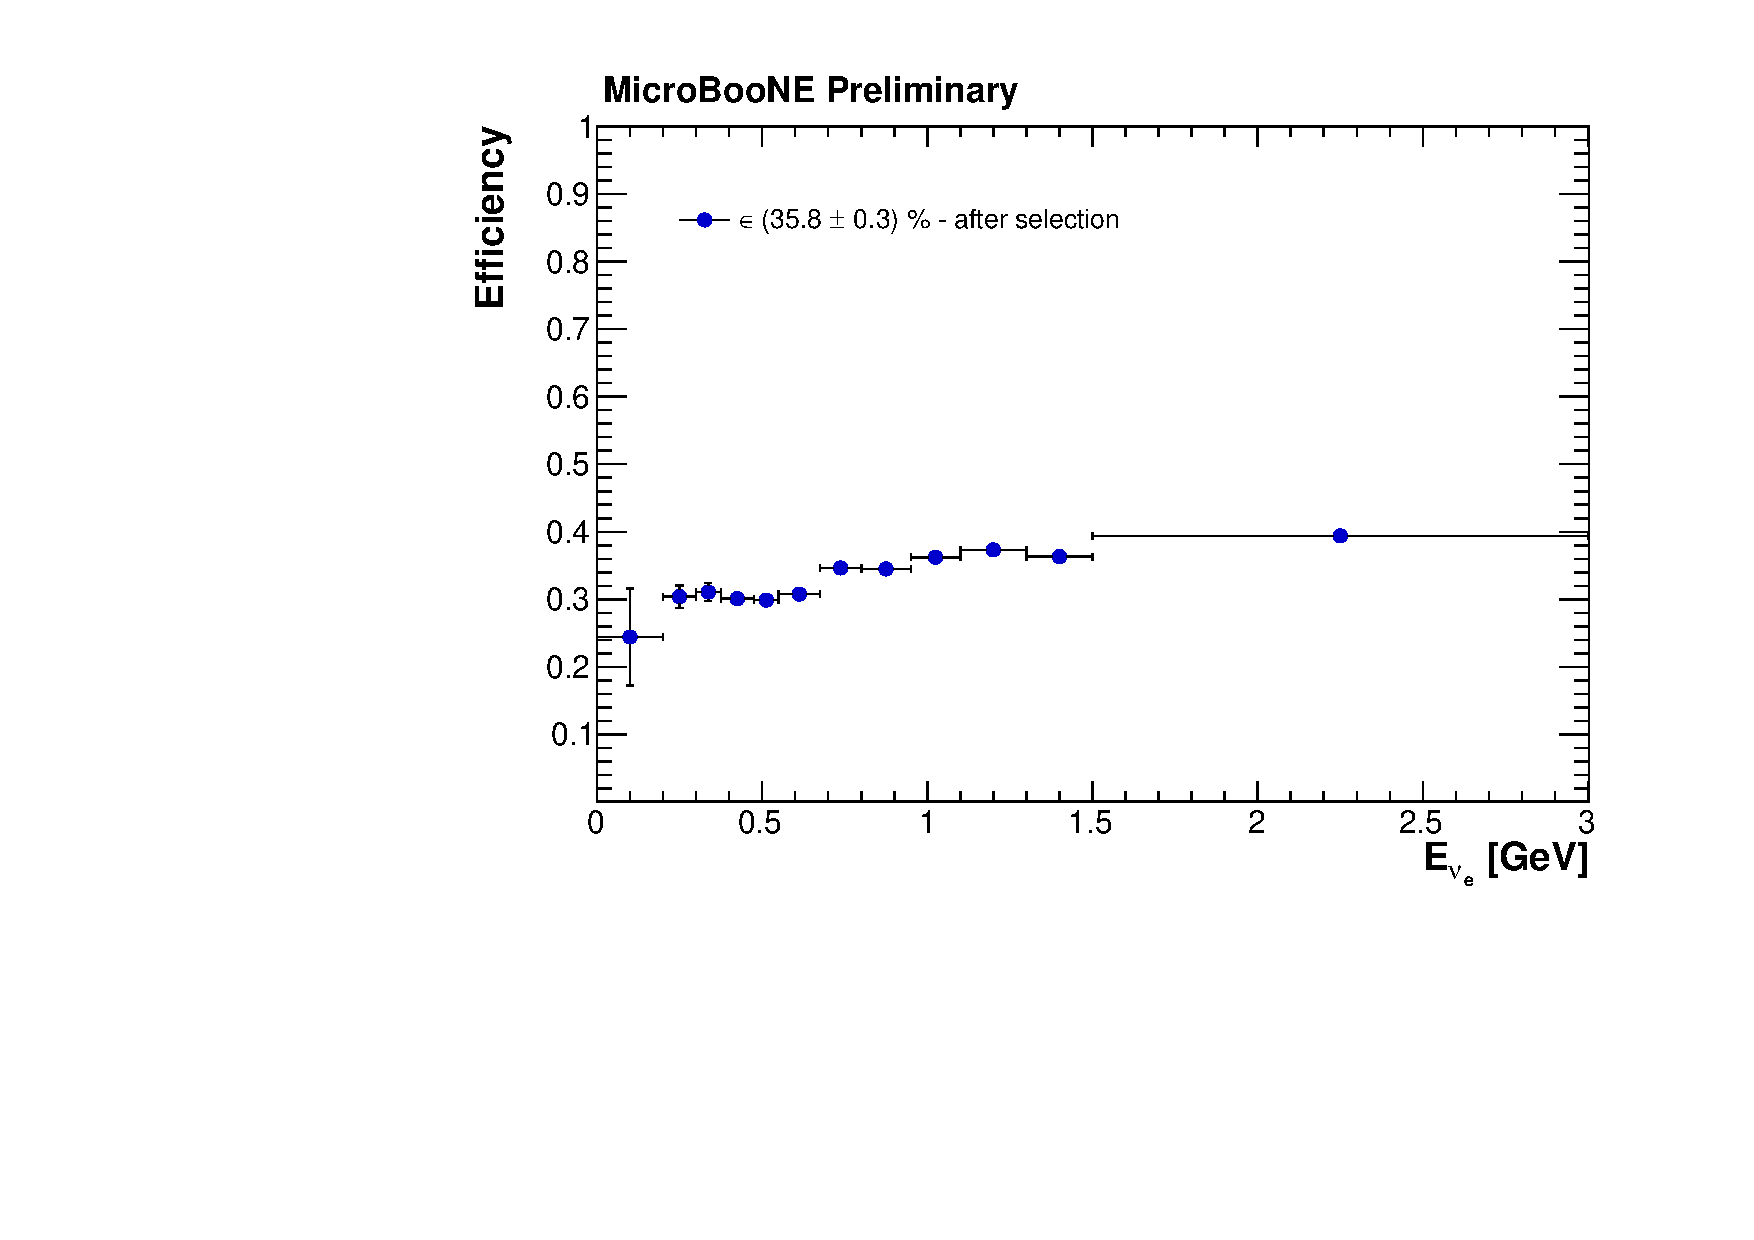
\includegraphics[width=\linewidth]{figures/eff.pdf}
    \caption{Efficiency} 
  \end{subfigure}
    \begin{subfigure}{0.48\textwidth}
    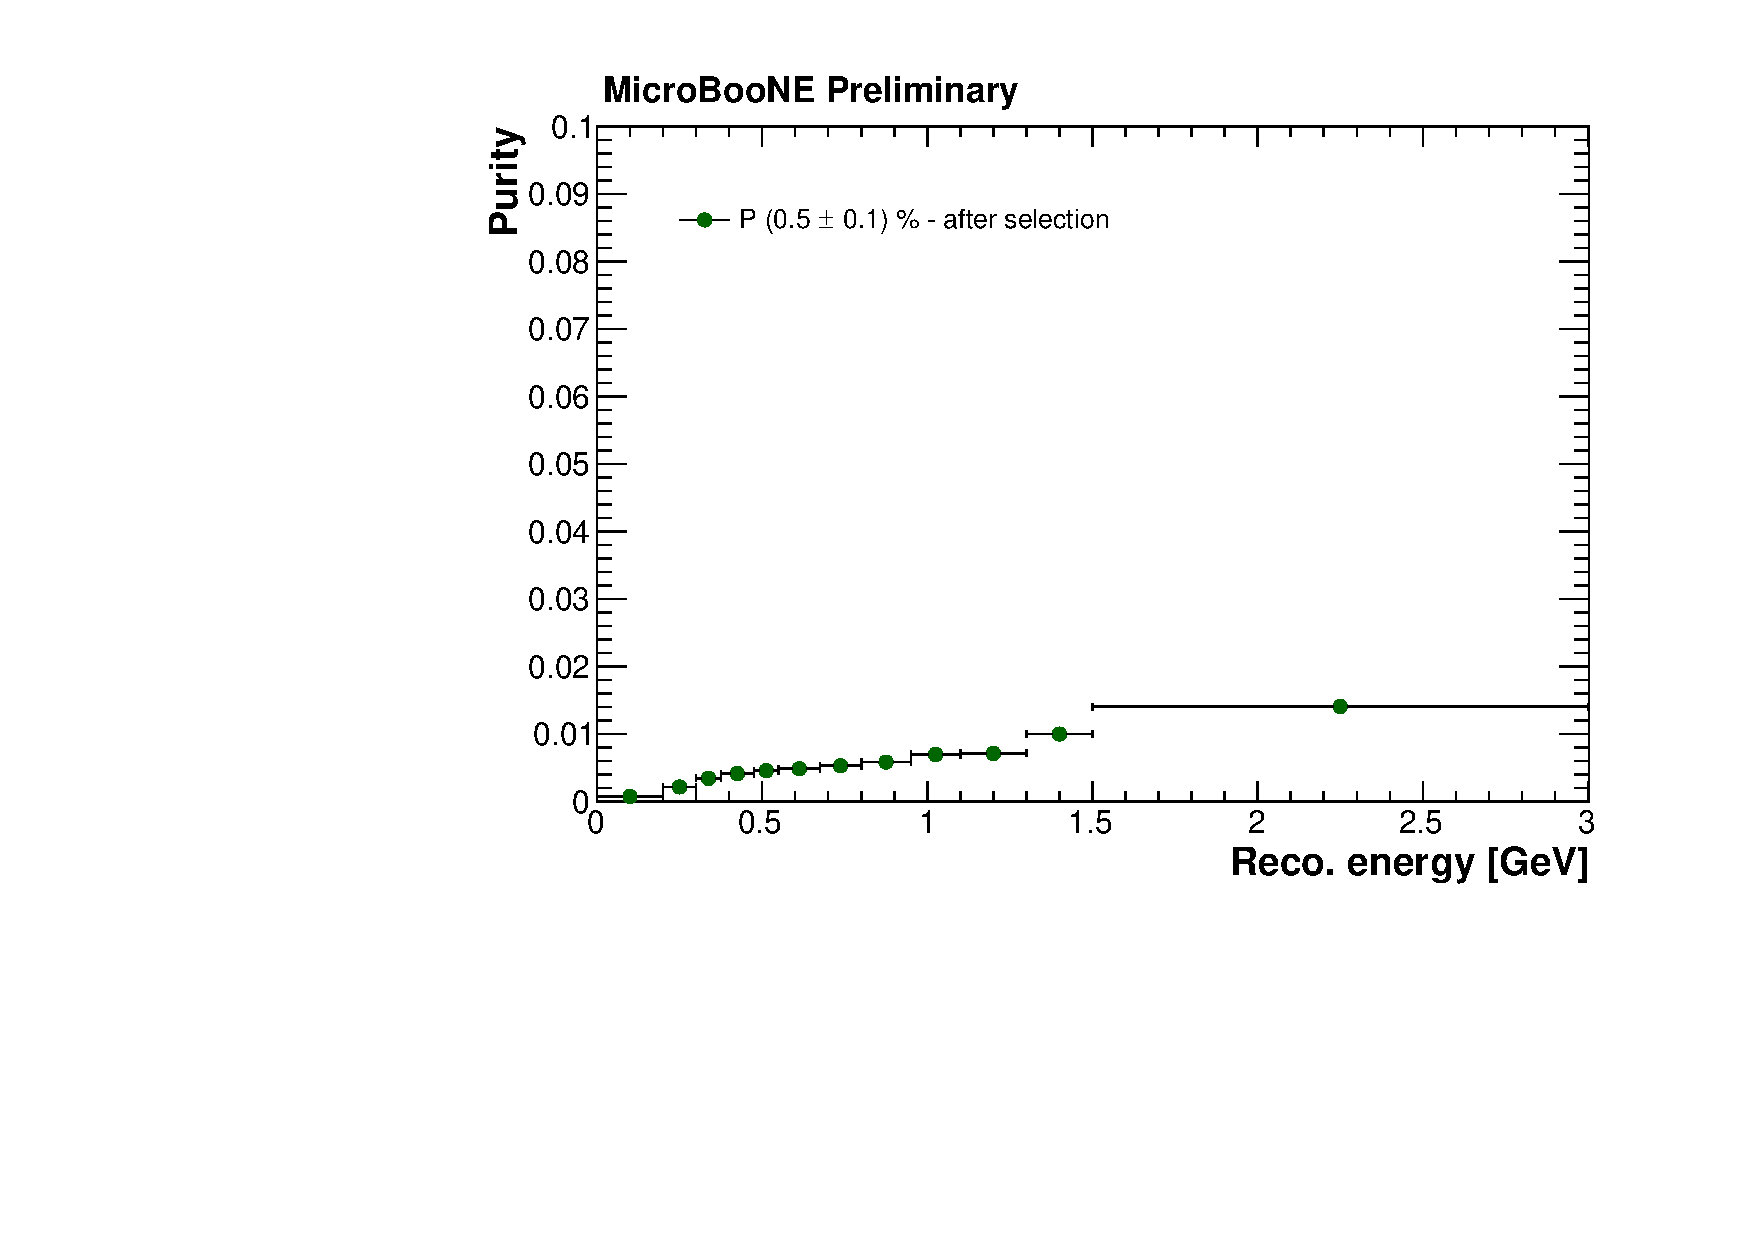
\includegraphics[width=\linewidth]{figures/purity.pdf}
    \caption{Purity} 
  \end{subfigure}
  \caption{Left: $\nu_{e}$ CC$0\pi$-Np reconstruction efficiency as a function of the true $\nu_{e}$ energy. Right: $\nu_{e}$ CC$0\pi$-Np purity as a function of the reconstructed energy.}
  \label{fig:effpurity}
\end{figure}

In order to understand the different background components, we divided our sample of selected events into further 8 categories:

\begin{itemize}
\item Beam intrinsic $\nu_{e}$ CC$0\pi$-Np: charged-current $\nu_{e}$ neutrino interaction with no pions in the final state and at least one proton (N > 1).
\item Beam intrinsic $\nu_{e}$ CC: charged-current $\nu_{e}$ neutrino interaction that is not in the $\nu_{e}$ CC$0\pi$-Np channel.
\item Beam intrinsic $\nu_{\mu}$: charged-current $\nu_{\mu}$ neutrino interaction.
\item Beam intrinsic NC: neutral current neutrino interaction (both $\nu_{\mu}$ and $\nu_{e}$).
\item Dirt: the neutrino interacts outside the TPC, but one or more final-state particles produce a neutrino candidate inside in the fiducial volume.
\item Cosmic: there is a neutrino interaction in the event, but the cosmic-ray interaction happening during the same drift time is selected instead.
\item Cosmic in-time: there is no neutrino interaction in the event and a cosmic-ray interaction happening inside the beam gate time window is selected. It corresponds to the data EXT sample.
\item Cosmic contaminated: the neutrino interaction candidate contains at least a track or a shower generated by a cosmic ray.

\end{itemize}

Table \ref{tab:result} shows a summary of the selection algorithm results, with the corresponding number of events for each category. The numbers correspond to an exposure of the MicroBooNE detector of \num{4.84e19} protons on target (POT), which is the amount of data available in the open sample.

\begin{table}[htbp]
   \centering
   \begin{tabular}{llrrrrr}
     \toprule
     Category & \phantom{a} & Generated & \phantom{a} & Selected & \phantom{a} & Efficiency \\
     \midrule

     $\nu_{e}$ CC0$\pi$-Np       & & 35.5     & & 12.7   & & 35.8\%\\
     $\nu_{e}$ CC                & & 35.7     & & 12.0   & & 33.6\%\\
     Beam intrinsic $\nu_{\mu}$  & & 11405.0  & & 805.8  & & 7.1\%\\
     Beam intrinsic NC           & & 3660.3   & & 299.8  & & 8.2\%\\
     Dirt                        & & 2651.1   & & 30.6   & & 1.2\%\\
     Cosmic in-time              & & 135377.2 & & 1086.7 & & 0.8\%\\
     Cosmic contaminated         & & -        & & 246.2  & & -\\
     Cosmic                      & & -        & & 280.2  & & -\\

     \bottomrule
   \end{tabular}
   \caption{Summary of the selection algorithm results, showing the contribution of each event category, for a MicroBooNE exposure of \num{4.84e19} POT.}\label{tab:result}
\end{table}

\subsection{Background rejection}\label{sec:cuts}
The very low purity of the sample obtained after the selection algorithm shows that it is necessary to improve the rejection of background events. 

\paragraph{Charged-current $\nu_{\mu}$ and cosmic-induced background rejection}
The module \texttt{UBXSec} \cite{ubxsec} looks for charged-current $\nu_{\mu}$ candidates and it also helps reject cosmic-induced background events.  Figure \ref{fig:spectrum} shows the reconstructed energy spectrum obtained vetoing the events that \texttt{UBXSec} flagged as CC $\nu_{\mu}$ candidates or cosmic-induced background (the reconstructed energy has been measured with the procedure described in Section \ref{sec:energyreco}). The ratio between the number of data events and the number of Monte Carlo events (POT normalized) is compatible with the unity (1.01) and the low value of the $\chi^{2} / \mathrm{n.d.f.}$ (0.29) shows that the two distributions agree also in shape.

\begin{figure}[htbp]
\centering
  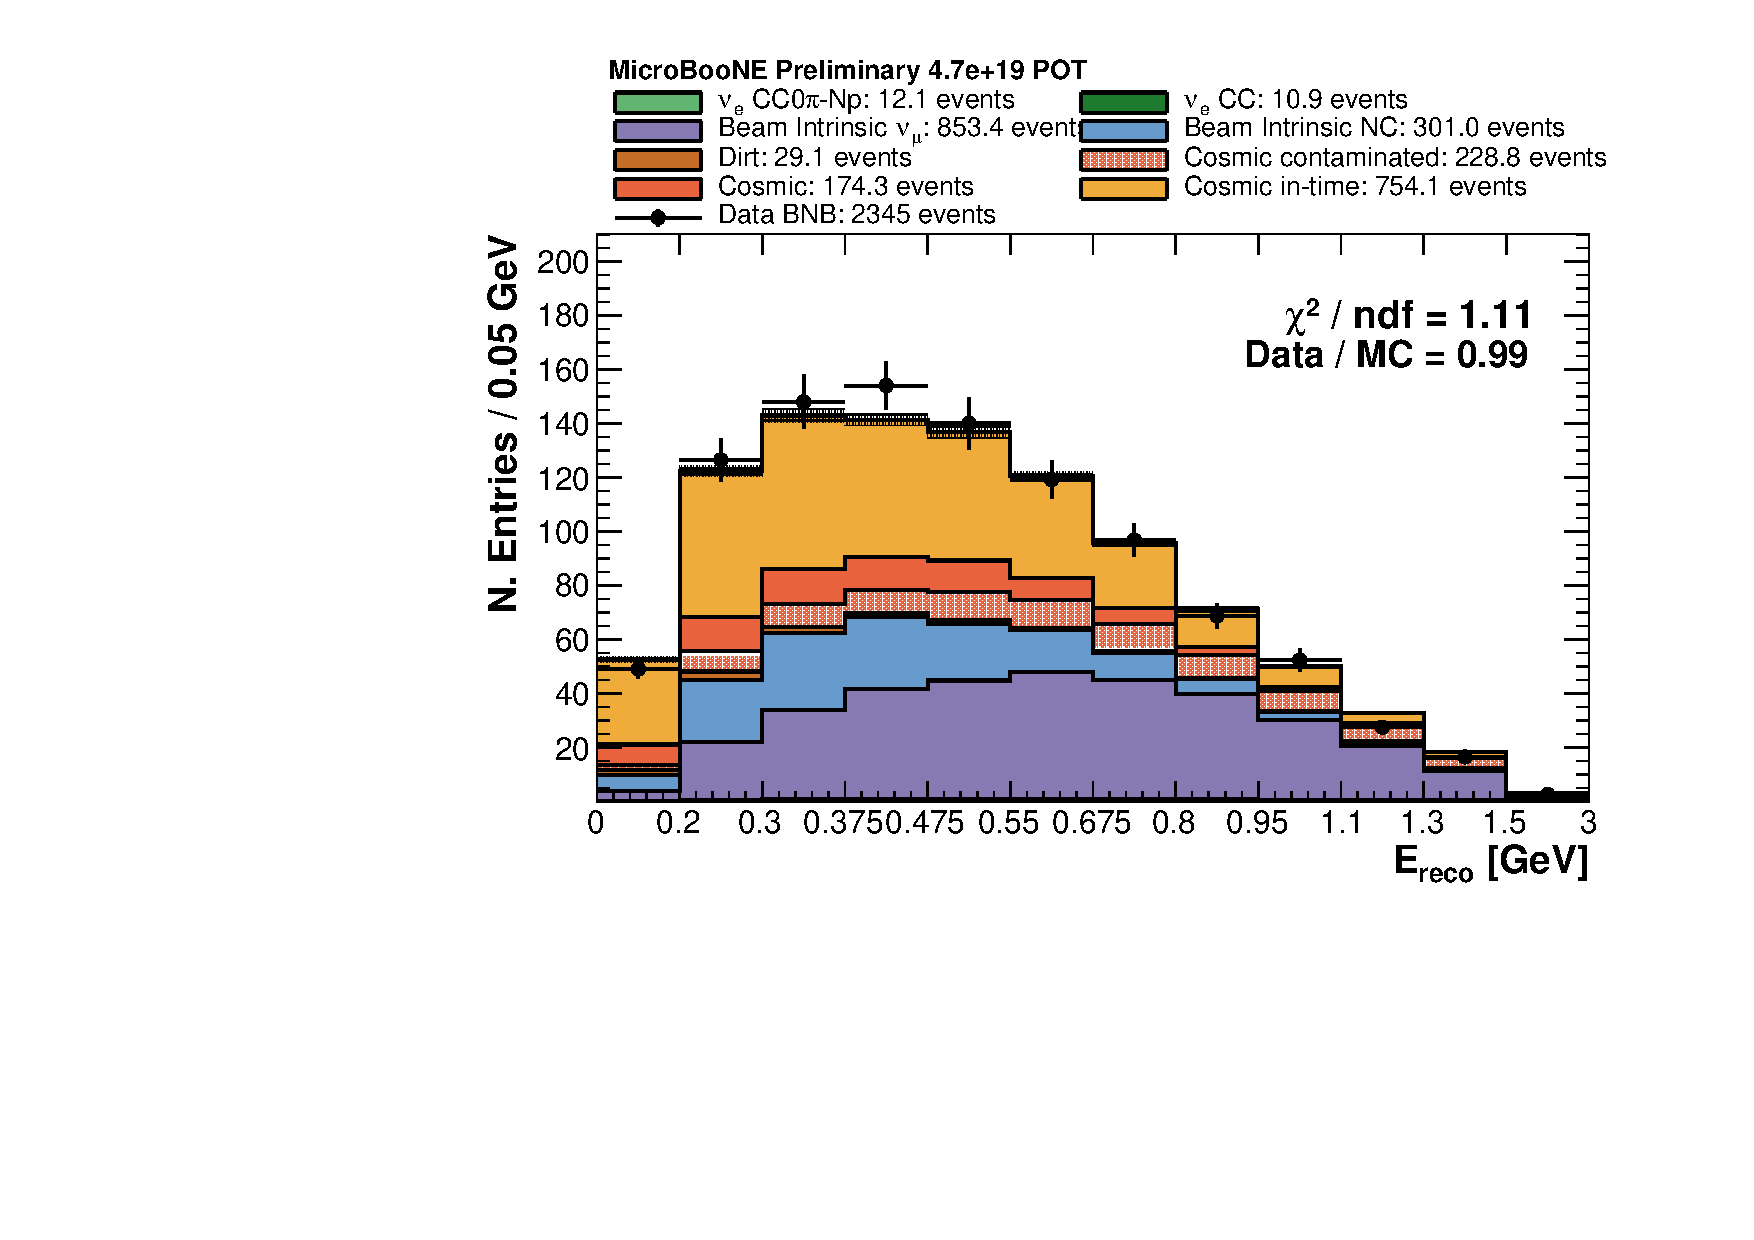
\includegraphics[width=0.7\linewidth]{figures/h_fixed_energy.pdf}
  \caption{Reconstructed energy spectrum after the event selection algorithm and the veto of the events selected by the \texttt{UBXSec} module. The histograms of the event categories are stacked.}
  \label{fig:spectrum}
\end{figure}

\paragraph{Shower energy cut}
The energy of each electromagnetic shower is measured with the procedure described in Section \ref{sec:showerenergy}. A large number of cosmic in-time events will have a low shower energy, mainly caused by Michel electrons. A significant portion of charged-current $\nu_{\mu}$ events will also have low-energy showers caused by stopping muons and spurious hits. A cut of 50 MeV on the reconstructed energy of the most energetic shower removes a large fraction of the cosmic in-time and CC $\nu_{\mu}$ backgrounds, without significantly reducing the $\nu_{e}$ CC0$\pi$-Np efficiency. Figure \ref{fig:showerenergy} shows the reconstructed energy distribution of the most energetic shower in the low-energy region and the reconstructed energy spectrum after the shower energy cut.

\paragraph{Shower $dE/dx$ cut}

\paragraph{Shower distance cut}

\paragraph{Track-shower angle cut}

\paragraph{Track $dQ/dx$ cut}

\paragraph{Shower opening angle cut}

\paragraph{Track length cut}


\section{Energy reconstruction}\label{sec:energyreco}
\subsection{Electron energy reconstruction and calibration}\label{sec:showerenergy}
The reconstructed energy $E_{reco}$ of a shower-like object is measured converting the charge of the associated hits into deposited energy in the TPC. It is calculated by multiplying the reconstructed charge ($e^{-}_{reco}$) from hits associated with the reconstructed shower by the calibration factor measured in \cite{michel}:
\begin{equation}
\frac{E_{reco} \mathrm{(MeV)}}{e^-} = 1.01\frac{e^-}{e^{-}_{reco}} \times \frac{23.6~\mathrm{eV}}{e^-} \times 10^{-6} \frac{\mathrm{eV}}{\mathrm{MeV}} \times \frac{1}{R},
\end{equation}
where:
\begin{itemize}

\item the correction factor $1.01\frac{e^-}{e^{-}_{reco}}$ is obtained measuring the true number of collected electrons $e^{-}$ on the wires using a sample of stopping muons, fitting the $dE/dx$ vs. residual range to values for argon as tabulated by the PDG \cite{pdg},
\item $\frac{23.6~\mathrm{eV}}{e^-}$ is the work function for ionizing an argon atom \cite{workfunction},
\item $R = 0.62$ is the recombination factor obtained with the Modified Box Model \cite{boxmodel}.
\end{itemize}
Figure \ref{fig:ecalib} shows the calibration slope necessary to convert the reconstructed energy $E_{reco}$ into true electron energy $E_{true}$. It has been obtained using only the hits reconstructed in the collection plane. 

\subsection{Proton energy reconstruction and calibration}


\subsection{\texorpdfstring{$\pi^0$}{pi0} mass peak}

CC$\pi^0$ events have been studied in order to validate the energy scale and reconstruction in the low-energy region in data as well as in the Monte Carlo. There is no aim for an analysis in the CC$\pi^0$ channel. Instead the purpose is to exploit a pure sample of $\pi^0$ decays, which can be used as standard candle to validate the energy reconstruction.
The samples which have been used are:
\begin{itemize}
  \item Data: hand scanned CC$\pi^0$ sample
  \item Monte Carlo: BNB + cosmic + generator level requirements:
  	\begin{itemize}
  		\item Selected neutrino matched to a true neutrino
		\item Charged current interaction
		\item Exactly one $\pi^0$ in the final state
  	\end{itemize}
\end{itemize}
The selection relies on the optical selection presented before (ref. to optical selection). Subsequently events are required to have at least two reconstructed showers with hits on the collection plane. The second requirement is meant to remove events with null shower energy, as the energy is computed from the collection plane only. The energy of the showers is calibrated using the energy calibration shown previously (derived from electrons-matched-showers using the Monte Carlo, ref. to this calibration).
The $\pi^0$ candidate is computed starting from the two most energetic showers. The distribution of the number of reconstructed showers in each event is shown in the left plot in fig. \ref{fig:mc_mass_e2} for data and MC.

As there are many events with more than two showers, about two thirds in data and one half in Monte Carlo, a simple re-clustering of the energy is performed. It is meant to recover the energy from broken showers. The two most energetic showers are considered. Then, the energy of any additional shower is summed to the closest in angle among the two most energetic showers. The direction of the two most energetic showers is not modified in this process. The mass is computed from the two most energetic showers, with the energy corrected after the re-clustering, as:
\[ M = \sqrt{E_1 E_2 (1 - \cos\theta)} \]\textbf{}
where $E_1$ and $E_2$ are the energies of the most and the second most energetic showers, respectively. $\theta$ is the 3-D angle between the directions of the two showers.

\begin{figure}[!htbp]
\centering
\begin{minipage}{0.49\columnwidth}
  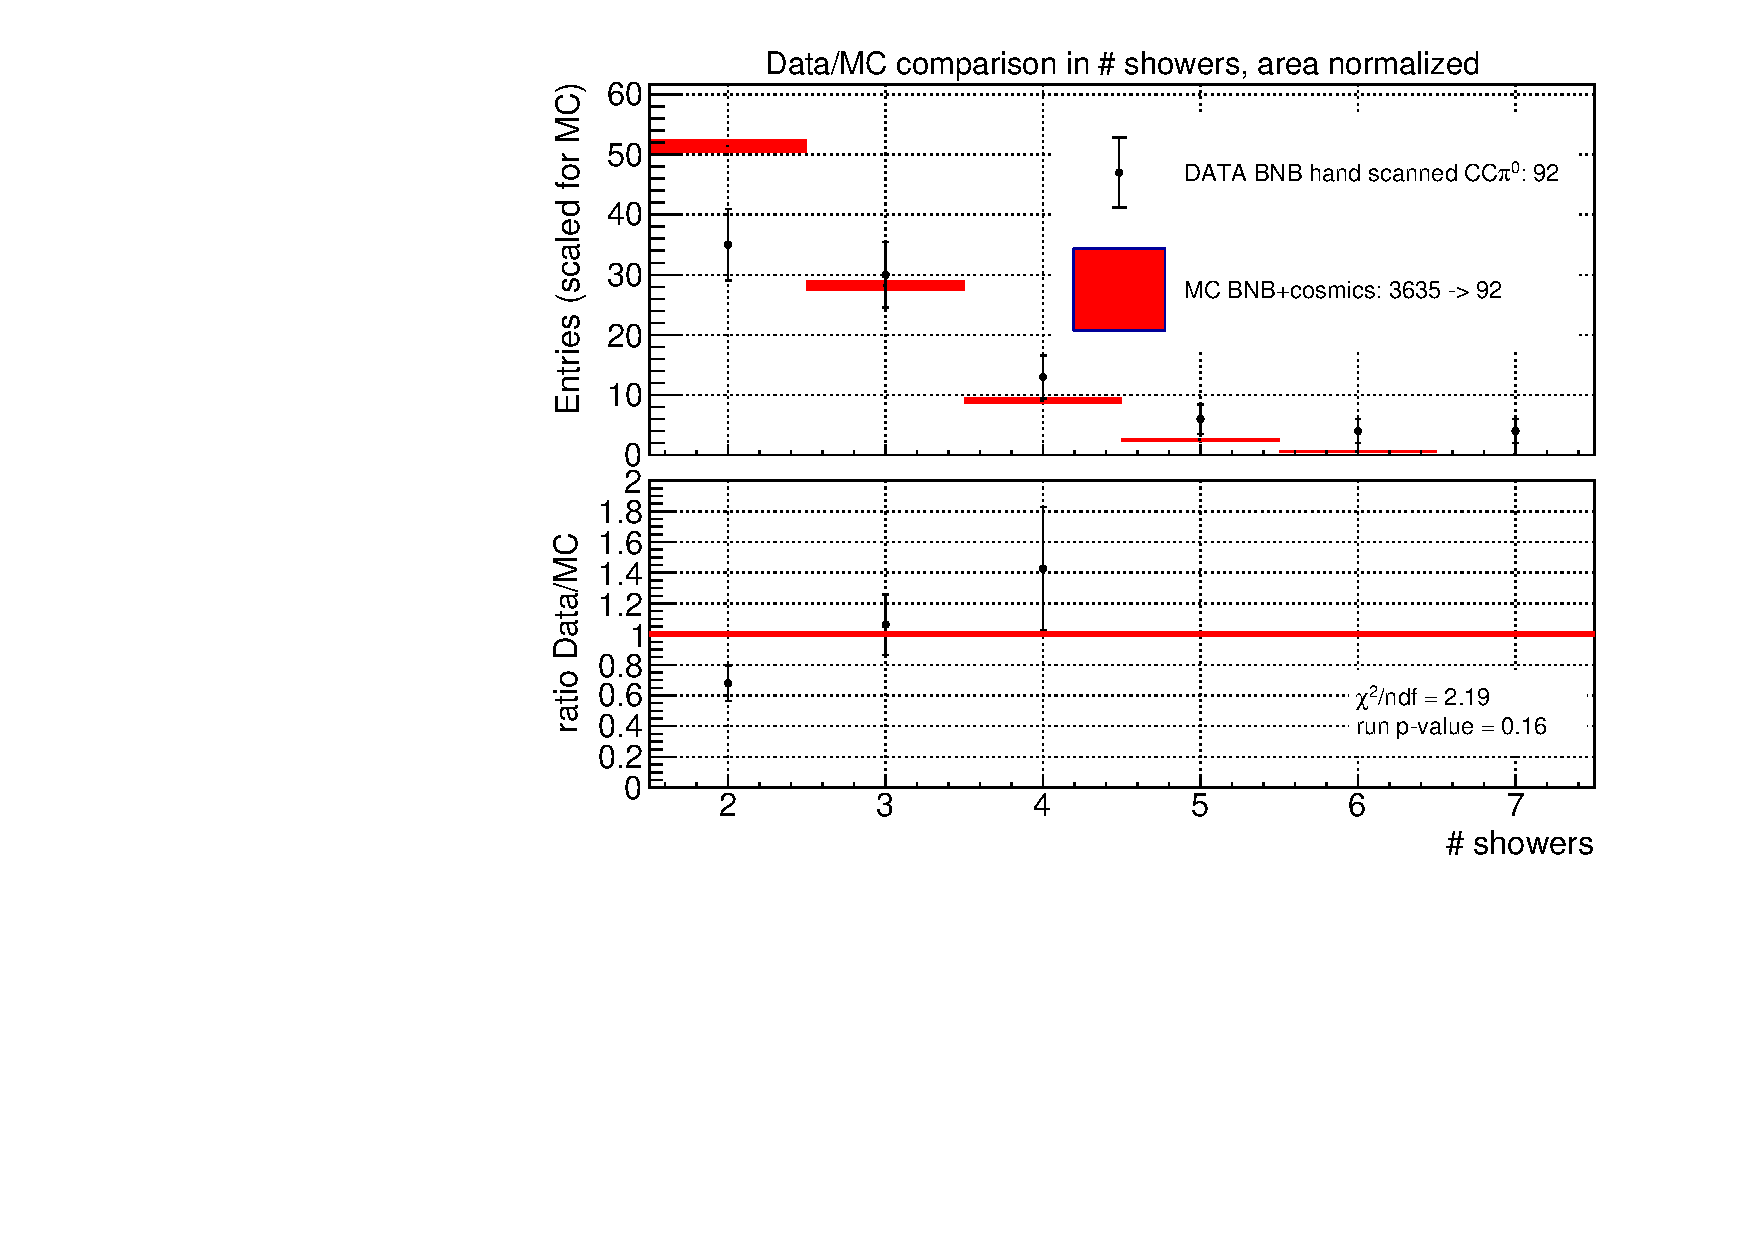
\includegraphics[width=0.99\columnwidth]{_fig/n_showers_data_MC_comparison.pdf}
\end{minipage}
\begin{minipage}{0.49\columnwidth} 
  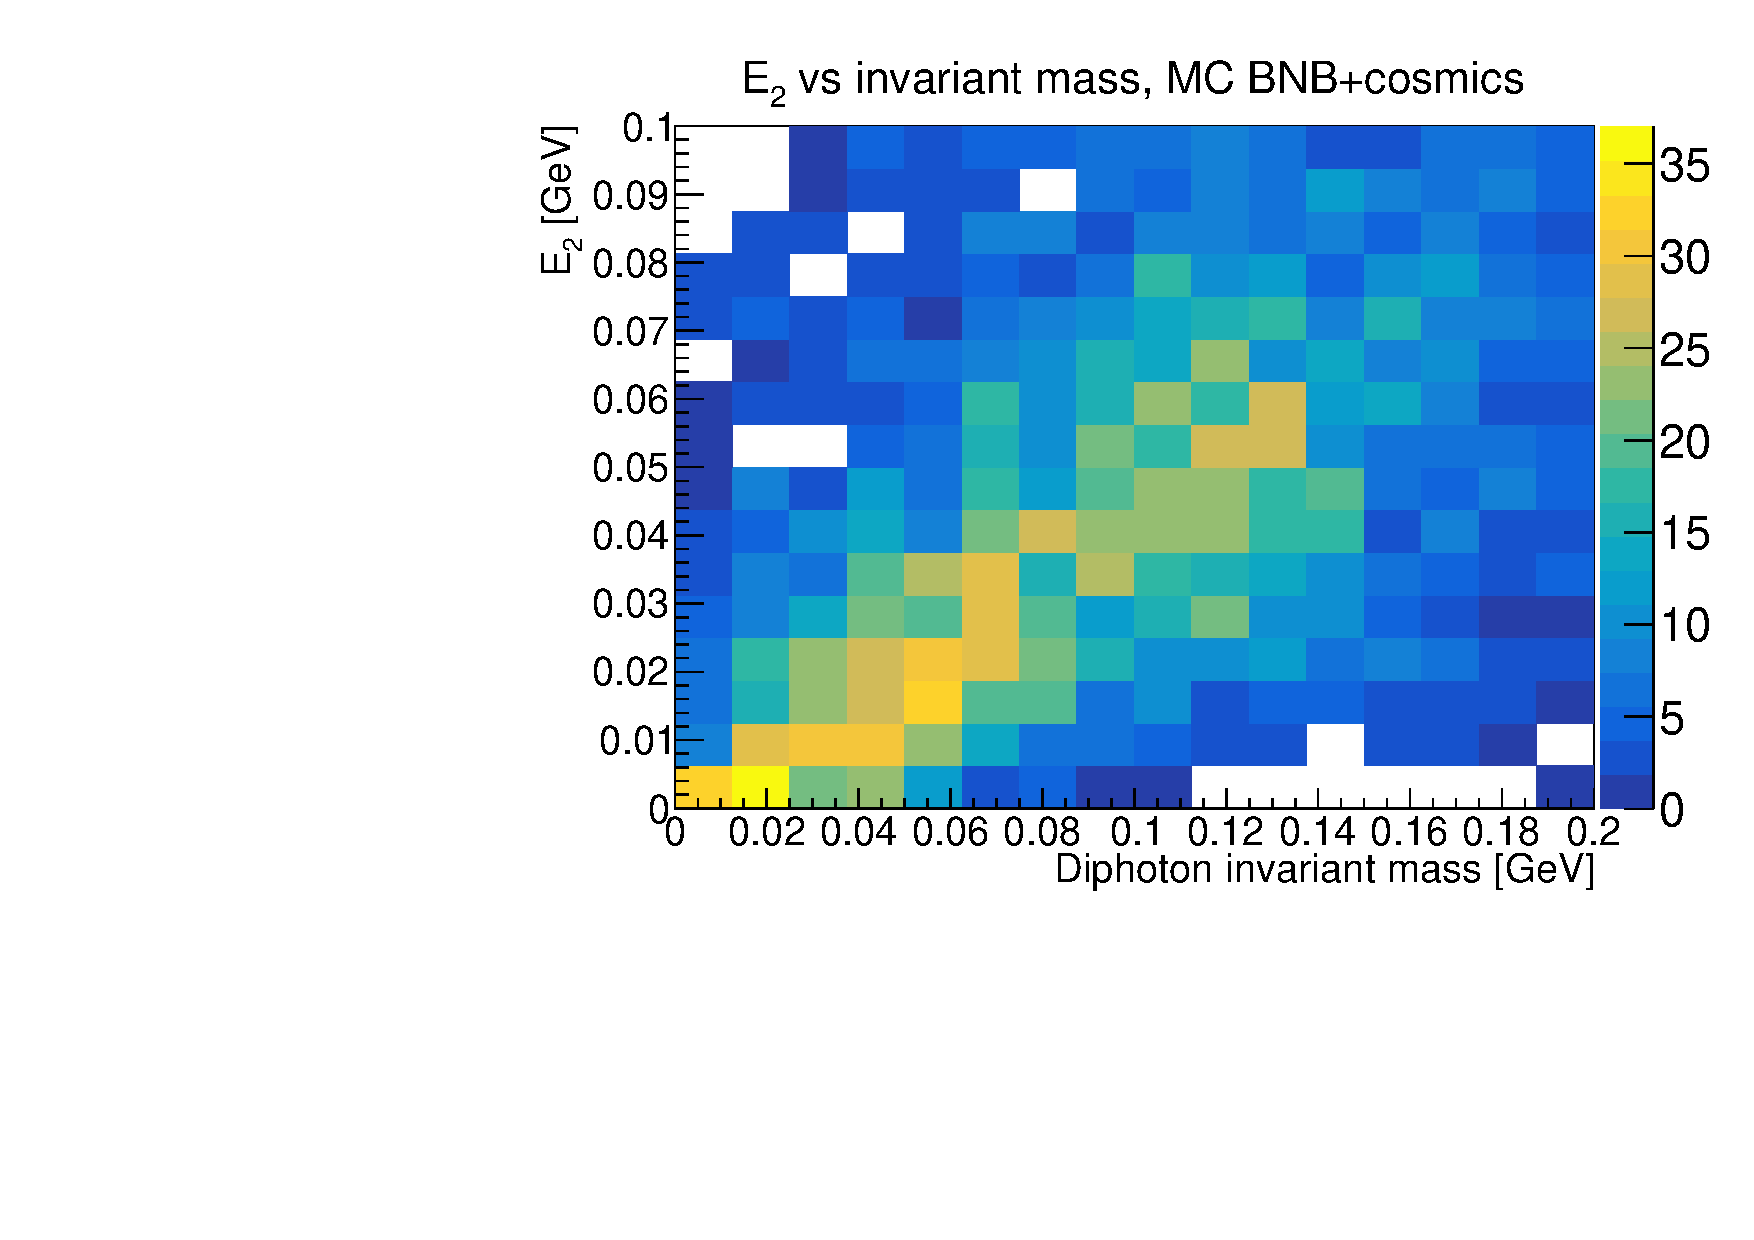
\includegraphics[width=0.99\columnwidth]{_fig/MC_mass_E2.pdf}
\end{minipage}
\caption{Left: Distribution of the number of showers for each event, for data (black dots) and Monte Carlo (red boxes). Right: Bi-dimensional distribution of $E_2$ (y-axis) versus the invariant mass (x-axis) in Monte Carlo events.}
\label{fig:mc_mass_e2}
\end{figure}

In some cases a significant amount of energy is missing. For instance one of the two true showers is missed, and a smaller showers, resulting from noise or from mis-reconstruction of other objects, is taken as one of the decay products of the $\pi^0$. The right plot in figure \ref{fig:mc_mass_e2} shows the bi-dimensional distribution of the invariant mass (x-axis) versus $E_2$ (x-axis) for Monte Carlo events. As it is possible to see, a significant amount of events has small $E_2$ and small mass. Thus, to take into account this effect and remove events with one shower badly or mis-reconstructed, the second most energetic shower is required to have reconstructed energy larger than 30 MeV.

The final peak after the selection is shown in figure \ref{fig:pi0_mass_peak}. The two histograms, for data and Monte Carlo, are fitted through a binned ML fit with a crystal ball function (Gaussian core, $C^1$-matched with a power-law right tail). The fit result, for what concerns the core is:
\[ \text{Data:} \quad \mu = 133 \pm 7~\text{MeV}, \quad \sigma = 47 \pm 5~\text{MeV} \]
\[ \text{Monte Carlo:} \quad \mu = 119 \pm 2~\text{MeV}, \quad \sigma = 51 \pm 2~\text{MeV} \]

The two results are significantly close to the nominal mass of 135~MeV, and shows a relatively good agreement between data and Monte Carlo. However, the discrepancy is significant and requires more investigation, in order to be understood completely.

\begin{figure}[!htbp]
\centering
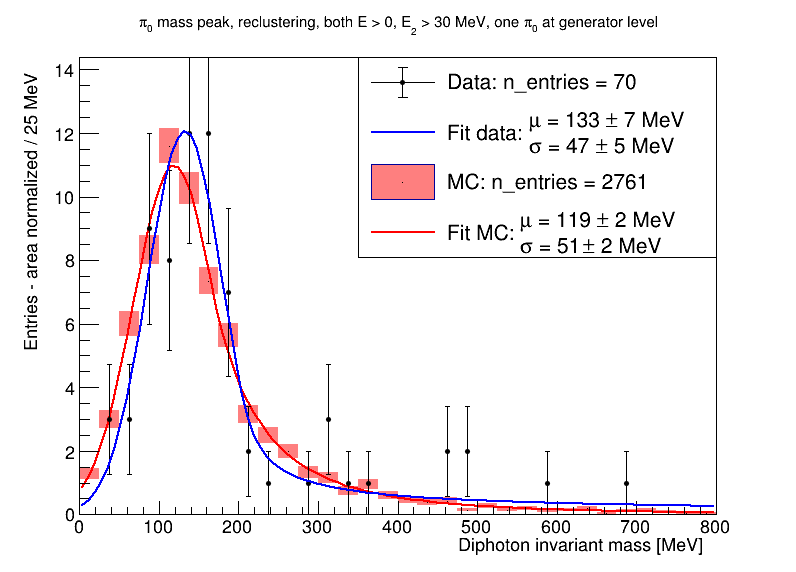
\includegraphics[width=0.8\textwidth]{_fig/data_mc_pi0_mass_peak_crb_cut_on_second_shower.png}
\caption{Diphoton invariant mass distribution for data and Monte Carlo. The two lines show the crystal ball functions as obtained from the ML fit to the two histrograms.} 
\label{fig:pi0_mass_peak}
\end{figure}


\begin{thebibliography}{99}

\bibitem{miniboone}
  A.~A.~Aguilar-Arevalo {\emph{et al.}} [MiniBooNE Collaboration],
  ``Unexplained Excess of Electron-Like Events From a 1-GeV Neutrino Beam,''
  Phys.\ Rev.\ Lett.\  \textbf{102} (2009) 101802
  doi:10.1103/PhysRevLett.102.101802
  \href{https://arxiv.org/abs/0812.2243}{\texttt{[arXiv:0812.2243 [hep-ex]]}}.
  %%CITATION = doi:10.1103/PhysRevLett.102.101802;%%
  %385 citations counted in INSPIRE as of 06 Dec 2017
  
\bibitem{icecube}
  M.~G.~Aartsen {\emph{et al.}} [IceCube Collaboration],
  ``Constraints on Ultrahigh-Energy Cosmic-Ray Sources from a Search for Neutrinos above 10 PeV with IceCube,''
  Phys.\ Rev.\ Lett.\  \textbf{117} (2016) no.24,  241101
  doi:10.1103/PhysRevLett.117.241101
  \href{https://arxiv.org/abs/1607.05886}{\texttt{[arXiv:1607.05886 [astro-ph.HE]]}}.
  %%CITATION = doi:10.1103/PhysRevLett.117.241101;%%
  %39 citations counted in INSPIRE as of 06 Dec 2017
  
\bibitem{Formaggio:2013kya}
  J.~A.~Formaggio and G.~P.~Zeller,
  ``From eV to EeV: Neutrino Cross Sections Across Energy Scales,''
  Rev.\ Mod.\ Phys.\  \textbf{84} (2012) 1307
  doi:10.1103/RevModPhys.84.1307
  \href{https://arxiv.org/abs/1305.7513}{\texttt{[arXiv:1305.7513 [hep-ex]]}}.
  %%CITATION = doi:10.1103/RevModPhys.84.1307;%%
  %221 citations counted in INSPIRE as of 08 Dec 2017
  
  
     \bibitem{nuecc}
  M.~Day and K.~S.~McFarland,
  ``Differences in Quasi-Elastic Cross-Sections of Muon and Electron Neutrinos,''
  Phys.\ Rev.\ D \textbf{86} (2012) 05300 
  doi:10.1103/PhysRevC.86.054606
  \href{https://arxiv.org/abs/1206.6745}{\texttt{[arXiv:1206.6745 [hep-ph]]}}.
  %%CITATION = doi:10.1103/PhysRevC.86.054606;%%
  %81 citations counted in INSPIRE as of 13 Dec 2017
  
  \bibitem{genie}
  C.~Andreopoulos \emph{et al.},
  ``The GENIE Neutrino Monte Carlo Generator,''
  Nucl.\ Instrum.\ Meth.\ A \textbf{ 614} (2010) 87
  doi:10.1016/j.nima.2009.12.009
  \href{https://arxiv.org/abs/0905.2517}{\texttt{[arXiv:0905.2517 [hep-ph]]}}.
  %%CITATION = doi:10.1016/j.nima.2009.12.009;%%
  %473 citations counted in INSPIRE as of 15 Dec 2017
  
  \bibitem{corsika} D.~Heck \emph{et al.},
  ``CORSIKA: A Monte Carlo code to simulate extensive air showers'', 1998,
  \texttt{FZKA-6019}.
  
    \bibitem{pandora2} R.~Acciarri \emph{et al.} [MicroBooNE Collaboration], ``The Pandora multi-algorithm approach to automated pattern recognition of cosmic-ray muon and neutrino events in the MicroBooNE detector'', \href{https://arxiv.org/abs/1708.03135}{\texttt{[arXiv:1708.03135 [physics.hep-ex]]}}, accepted by Eur. Phys. J. C.
  
  \bibitem{ccqe2}
  M.~Martini and M.~Ericson,
  ``Quasielastic and multinucleon excitations in antineutrino-nucleus interactions,''
  Phys.\ Rev.\ C \textbf{87} (2013) no.6,  065501
  doi:10.1103/PhysRevC.87.065501
  \href{https://arxiv.org/abs/1303.7199}{\texttt{[arXiv:1303.7199 [nucl-th]]}}.
  %%CITATION = doi:10.1103/PhysRevC.87.065501;%%
  %59 citations counted in INSPIRE as of 13 Dec 2017
  
  \bibitem{pandora} J.~S.~Marshall and M.~A.~Thomson, 
  ``The Pandora Software Development Kit for Pattern Recognition'', Eur.\ Phys.\ J.\ C \textbf{75}, no. 9, 439 (2015) doi:10.1140/epjc/s10052\-015-3659-3 \href{https://arxiv.org/abs/1506.05348}{\texttt{[arXiv:1506.05348 [physics.data-an]]}}.
  

  


  \bibitem{teppei}
  T.~Katori [MiniBooNE and SciBooNE Collaborations],
  %``Cross section analyses in MiniBooNE and SciBooNE experiments,''
  AIP Conf.\ Proc.\  \textbf{ 1663} (2015) 020001
  doi:10.1063/1.4919461
  \href{https://arxiv.org/abs/1304.5325}{\texttt{[arXiv:1304.5325 [hep-ex]]}}.
  %%CITATION = doi:10.1063/1.4919461;%%
  %5 citations counted in INSPIRE as of 17 Jan 2018
  
 \bibitem{argoneut}
  R.~Acciarri \emph{et al.} [ArgoNeuT Collaboration],
  ``First Observation of Low Energy Electron Neutrinos in a Liquid Argon Time Projection Chamber,''
  Phys.\ Rev.\ D \textbf{ 95} (2017) no.7,  072005
  doi:10.1103/PhysRevD.95.072005
  \href{https://arxiv.org/abs/1610.04102}{\texttt{[arXiv:1610.04102 [hep-ex]]}}.
  %%CITATION = doi:10.1103/PhysRevD.95.072005;%%
  %5 citations counted in INSPIRE as of 20 Dec 2017
  
  \bibitem{proton}
  R.~Acciarri \emph{et al.} [MicroBooNE Collaboration],
  ``Proton Track Identication in MicroBooNE Simulation for Neutral Current Elastic Events,'' MICROBOONE-NOTE-1025-PUB,
  \url{http://microboone.fnal.gov/wp-content/uploads/MICROBOONE-NOTE-1025-PUB.pdf}.

  \bibitem{ubxsec}
  R.~Acciarri \emph{et al.} [MicroBooNE Collaboration],
  ``Muon-Neutrino Charged-Current Inclusive Analysis,'' \emph{in preparation}.

\bibitem{michel} 
  R.~Acciarri {\it et al.} [MicroBooNE Collaboration],
  ``Michel Electron Reconstruction Using Cosmic-Ray Data from the MicroBooNE LArTPC,''
  JINST {\bf 12}, no. 09, P09014 (2017)
  doi:10.1088/1748-0221/12/09/P09014
  \href{https://arxiv.org/abs/1704.02927}{\texttt{[arXiv:1704.02927 [physics.ins-det]]}}.
  %%CITATION = doi:10.1088/1748-0221/12/09/P09014;%%
  %6 citations counted in INSPIRE as of 09 Apr 2018

\bibitem{pdg} Particle Data Group, ``Atomic and nuclear properties of liquid argon (Ar)'' \url{http://pdg.lbl.gov/2012/AtomicNuclearProperties/MUON_ELOSS_TABLES/muonloss_289.pdf}, retrieved Apr. 9, 2018

\bibitem{workfunction} M.E. Shibamura et al., ``Drift velocities of electrons, saturation characteristics of ionization and W-values for conversion electrons in liquid argon, liquid argon-gas mixtures and liquid xenon'', Nucl. Instrumentation Meth., 131, (1975) p249

\bibitem{boxmodel} R. Acciarri et al., [ArgoNeuT Collaboration], ``A study of electron recombination using highly ionizing particles in the ArgoNeuT Liquid Argon TPC'', JINST {\bf 8} (2013) P08005
558 \href{https://arxiv.org/abs/1306.1712}{\texttt{arXiv:1306.1712 [hep-ex]}}.

\end{thebibliography}
% \subsection{How to add Citations and a References List}

% You can upload a \verb|.bib| file containing your BibTeX entries, created with JabRef; or import your \href{https://www.overleaf.com/blog/184}{Mendeley}, CiteULike or Zotero library as a \verb|.bib| file. You can then cite entries from it, like this: \cite{greenwade93}. Just remember to specify a bibliography style, as well as the filename of the \verb|.bib|.


% \bibliographystyle{alpha}
% \bibliography{sample}

\end{document}